%%%%%%%%%%%%%%%%%%%%%%%%%%%%%%%%%%%%%%%%%
% Masters/Doctoral Thesis 
% LaTeX Template
% Version 2.5 (27/8/17)
%
% This template was downloaded from:
% http://www.LaTeXTemplates.com
%
% Version 2.x major modifications by:
% Vel (vel@latextemplates.com)
%
% This template is based on a template by:
% Steve Gunn (http://users.ecs.soton.ac.uk/srg/softwaretools/document/templates/)
% Sunil Patel (http://www.sunilpatel.co.uk/thesis-template/)
%
% Template license:
% CC BY-NC-SA 3.0 (http://creativecommons.org/licenses/by-nc-sa/3.0/)
%
%%%%%%%%%%%%%%%%%%%%%%%%%%%%%%%%%%%%%%%%%

%----------------------------------------------------------------------------------------
%	PACKAGES AND OTHER DOCUMENT CONFIGURATIONS
%----------------------------------------------------------------------------------------

\documentclass[
11pt, % The default document font size, options: 10pt, 11pt, 12pt
%oneside, % Two side (alternating margins) for binding by default, uncomment to switch to one side
english, % ngerman for German
singlespacing, % Single line spacing, alternatives: onehalfspacing or doublespacing
%draft, % Uncomment to enable draft mode (no pictures, no links, overfull hboxes indicated)
%nolistspacing, % If the document is onehalfspacing or doublespacing, uncomment this to set spacing in lists to single
%liststotoc, % Uncomment to add the list of figures/tables/etc to the table of contents
%toctotoc, % Uncomment to add the main table of contents to the table of contents
%parskip, % Uncomment to add space between paragraphs
%nohyperref, % Uncomment to not load the hyperref package
headsepline, % Uncomment to get a line under the header
%chapterinoneline, % Uncomment to place the chapter title next to the number on one line
%consistentlayout, % Uncomment to change the layout of the declaration, abstract and acknowledgements pages to match the default layout
]{MastersDoctoralThesis} % The class file specifying the document structure

\usepackage[utf8]{inputenc} % Required for inputting international characters
\usepackage[T1]{fontenc} % Output font encoding for international characters

\usepackage{mathpazo} % Use the Palatino font by default

\usepackage[backend=bibtex,style=authoryear,natbib=true]{biblatex} % Use the bibtex backend with the authoryear citation style (which resembles APA)

\addbibresource{master.bib} % The filename of the bibliography

\usepackage[autostyle=true]{csquotes} % Required to generate language-dependent quotes in the bibliography

%----------------------------------------------------------------------------------------
%	MARGIN SETTINGS
%----------------------------------------------------------------------------------------

\geometry{
	paper=a4paper, % Change to letterpaper for US letter
	inner=2.5cm, % Inner margin
	outer=3.8cm, % Outer margin
	bindingoffset=.5cm, % Binding offset
	top=1.5cm, % Top margin
	bottom=1.5cm, % Bottom margin
	%showframe, % Uncomment to show how the type block is set on the page
}

%----------------------------------------------------------------------------------------
%	THESIS INFORMATION
%----------------------------------------------------------------------------------------

\thesistitle{Thesis Title} % Your thesis title, this is used in the title and abstract, print it elsewhere with \ttitle
\supervisor{Dr. James \textsc{Smith}} % Your supervisor's name, this is used in the title page, print it elsewhere with \supname
\examiner{} % Your examiner's name, this is not currently used anywhere in the template, print it elsewhere with \examname
\degree{Doctor of Philosophy} % Your degree name, this is used in the title page and abstract, print it elsewhere with \degreename
\author{John \textsc{Smith}} % Your name, this is used in the title page and abstract, print it elsewhere with \authorname
\addresses{} % Your address, this is not currently used anywhere in the template, print it elsewhere with \addressname

\subject{Biological Sciences} % Your subject area, this is not currently used anywhere in the template, print it elsewhere with \subjectname
\keywords{} % Keywords for your thesis, this is not currently used anywhere in the template, print it elsewhere with \keywordnames
\university{\href{http://www.university.com}{University Name}} % Your university's name and URL, this is used in the title page and abstract, print it elsewhere with \univname
\department{\href{http://department.university.com}{Department or School Name}} % Your department's name and URL, this is used in the title page and abstract, print it elsewhere with \deptname
\group{\href{http://researchgroup.university.com}{Research Group Name}} % Your research group's name and URL, this is used in the title page, print it elsewhere with \groupname
\faculty{\href{http://faculty.university.com}{Faculty Name}} % Your faculty's name and URL, this is used in the title page and abstract, print it elsewhere with \facname

\AtBeginDocument{
\hypersetup{pdftitle=\ttitle} % Set the PDF's title to your title
\hypersetup{pdfauthor=\authorname} % Set the PDF's author to your name
\hypersetup{pdfkeywords=\keywordnames} % Set the PDF's keywords to your keywords
}

\begin{document}

\frontmatter % Use roman page numbering style (i, ii, iii, iv...) for the pre-content pages

\pagestyle{plain} % Default to the plain heading style until the thesis style is called for the body content

%----------------------------------------------------------------------------------------
%	TITLE PAGE
%----------------------------------------------------------------------------------------

\begin{titlepage}
\begin{center}

\vspace*{.06\textheight}
{\scshape\LARGE \univname\par}\vspace{1.5cm} % University name
\textsc{\Large Doctoral Thesis}\\[0.5cm] % Thesis type

\HRule \\[0.4cm] % Horizontal line
{\huge \bfseries \ttitle\par}\vspace{0.4cm} % Thesis title
\HRule \\[1.5cm] % Horizontal line
 
\begin{minipage}[t]{0.4\textwidth}
\begin{flushleft} \large
\emph{Author:}\\
\href{http://www.johnsmith.com}{\authorname} % Author name - remove the \href bracket to remove the link
\end{flushleft}
\end{minipage}
\begin{minipage}[t]{0.4\textwidth}
\begin{flushright} \large
\emph{Supervisor:} \\
\href{http://www.jamessmith.com}{\supname} % Supervisor name - remove the \href bracket to remove the link  
\end{flushright}
\end{minipage}\\[3cm]
 
\vfill

\large \textit{A thesis submitted in fulfillment of the requirements\\ for the degree of \degreename}\\[0.3cm] % University requirement text
\textit{in the}\\[0.4cm]
\groupname\\\deptname\\[2cm] % Research group name and department name
 
\vfill

{\large \today}\\[4cm] % Date
%\includegraphics{Logo} % University/department logo - uncomment to place it
 
\vfill
\end{center}
\end{titlepage}

%----------------------------------------------------------------------------------------
%	DECLARATION PAGE
%----------------------------------------------------------------------------------------

\begin{declaration}
\addchaptertocentry{\authorshipname} % Add the declaration to the table of contents
\noindent I, \authorname, declare that this thesis titled, \enquote{\ttitle} and the work presented in it are my own. I confirm that:

\begin{itemize} 
\item This work was done wholly or mainly while in candidature for a research degree at this University.
\item Where any part of this thesis has previously been submitted for a degree or any other qualification at this University or any other institution, this has been clearly stated.
\item Where I have consulted the published work of others, this is always clearly attributed.
\item Where I have quoted from the work of others, the source is always given. With the exception of such quotations, this thesis is entirely my own work.
\item I have acknowledged all main sources of help.
\item Where the thesis is based on work done by myself jointly with others, I have made clear exactly what was done by others and what I have contributed myself.\\
\end{itemize}
 
\noindent Signed:\\
\rule[0.5em]{25em}{0.5pt} % This prints a line for the signature
 
\noindent Date:\\
\rule[0.5em]{25em}{0.5pt} % This prints a line to write the date
\end{declaration}

\cleardoublepage

%----------------------------------------------------------------------------------------
%	QUOTATION PAGE
%----------------------------------------------------------------------------------------

\vspace*{0.2\textheight}

\noindent\enquote{\itshape Thanks to my solid academic training, today I can write hundreds of words on virtually any topic without possessing a shred of information, which is how I got a good job in journalism.}\bigbreak

\hfill Dave Barry

%----------------------------------------------------------------------------------------
%	ABSTRACT PAGE
%----------------------------------------------------------------------------------------

\begin{abstract}
\addchaptertocentry{\abstractname} % Add the abstract to the table of contents
The Thesis Abstract is written here (and usually kept to just this page). The page is kept centered vertically so can expand into the blank space above the title too\ldots
\end{abstract}

%----------------------------------------------------------------------------------------
%	ACKNOWLEDGEMENTS
%----------------------------------------------------------------------------------------

\begin{acknowledgements}
\addchaptertocentry{\acknowledgementname} % Add the acknowledgements to the table of contents
The acknowledgments and the people to thank go here, don't forget to include your project advisor\ldots
\end{acknowledgements}

%----------------------------------------------------------------------------------------
%	LIST OF CONTENTS/FIGURES/TABLES PAGES
%----------------------------------------------------------------------------------------

\tableofcontents % Prints the main table of contents

\listoffigures % Prints the list of figures

\listoftables % Prints the list of tables

%----------------------------------------------------------------------------------------
%	ABBREVIATIONS
%----------------------------------------------------------------------------------------

\begin{abbreviations}{ll} % Include a list of abbreviations (a table of two columns)

\textbf{LAH} & \textbf{L}ist \textbf{A}bbreviations \textbf{H}ere\\
\textbf{WSF} & \textbf{W}hat (it) \textbf{S}tands \textbf{F}or\\

\end{abbreviations}

%----------------------------------------------------------------------------------------
%	PHYSICAL CONSTANTS/OTHER DEFINITIONS
%----------------------------------------------------------------------------------------

\begin{constants}{lr@{${}={}$}l} % The list of physical constants is a three column table

% The \SI{}{} command is provided by the siunitx package, see its documentation for instructions on how to use it

Speed of Light & $c_{0}$ & \SI{2.99792458e8}{\meter\per\second} (exact)\\
%Constant Name & $Symbol$ & $Constant Value$ with units\\

\end{constants}

%----------------------------------------------------------------------------------------
%	SYMBOLS
%----------------------------------------------------------------------------------------

\begin{symbols}{lll} % Include a list of Symbols (a three column table)

$a$ & distance & \si{\meter} \\
$P$ & power & \si{\watt} (\si{\joule\per\second}) \\
%Symbol & Name & Unit \\

\addlinespace % Gap to separate the Roman symbols from the Greek

$\omega$ & angular frequency & \si{\radian} \\

\end{symbols}

%----------------------------------------------------------------------------------------
%	DEDICATION
%----------------------------------------------------------------------------------------

\dedicatory{For/Dedicated to/To my\ldots} 

%----------------------------------------------------------------------------------------
%	THESIS CONTENT - CHAPTERS
%----------------------------------------------------------------------------------------

\mainmatter % Begin numeric (1,2,3...) page numbering

\pagestyle{thesis} % Return the page headers back to the "thesis" style

% Include the chapters of the thesis as separate files from the Chapters folder
% Uncomment the lines as you write the chapters

% Chapter 1

\chapter{Introduction} % Main chapter title

\label{Chapter1} % For referencing the chapter elsewhere, use \ref{Chapter1} 

%----------------------------------------------------------------------------------------

% Define some commands to keep the formatting separated from the content 
\newcommand{\keyword}[1]{\textbf{#1}}
\newcommand{\tabhead}[1]{\textbf{#1}}
\newcommand{\code}[1]{\texttt{#1}}
\newcommand{\file}[1]{\texttt{\bfseries#1}}
\newcommand{\option}[1]{\texttt{\itshape#1}}

%----------------------------------------------------------------------------------------

\section{Background to the problem}
A software system is constantly subject to change pressure from its environment, therefore it needs to evolve to deliver value to its stakeholders throughout its lifetime: it has been regarded at least since the 1980's that software evolution is the most expensive part of the software lifecycle (Lehman, 1980). Therefore, an understanding of the capacity of a system to adapt to changes in its environment can impact on the software production process (Yu and Ramaswamy, 2006).

Open source development challenges traditional best practices in software development by blurring the difference between users and developers (Hippel and Krogh, 2003). The open source development model originated in the academic community and has transcended into private enterprise, where in many cases it has proven an efficient alternative to strong intellectual property protection (Kogut and Metiu, 2001).

Common tasks in software evolution include cloning, branching and merging of the code base; in addition to these processes, the open source license grants the freedom to fork a project: open source projects can evolve in parallel, splitting in two or more different projects, steered by different development teams.

The gain in popularity of the open source development model has brought forward the importance of understanding forking processes. Kogut and Metiu (2001) argue that forking results in competing versions of the original project and that forking is therefore a major failure risk for open source projects. Nyman and Lindman (2013) argue that forking is a remedy against ailments of proprietary software (planned obsolescence, vendor lock-in, hostile takeovers, etc.) and that forking facilitates experimentation. Robles and González-Barahona (2012) suggest that a purposeful fork can solve technical-, license- and team-related problems by restoring the balance between the stakeholders of a project. Therefore, a controversy exists within the software engineering community, whether forking is a risk or an opportunity.

%----------------------------------------------------------------------------------------

\section{Justification for the research}

Concepts in software evolution and biological evolution are often described using a common vocabulary (Yu and Ramaswamy, 2006), so it seems natural to look at evolutionary biology for potential methods to solve this controversy.

Lehman (1980) postulates that there are recurring patterns which govern software evolution, independently of the decisions taken by individual managers and programmers. Therefore, software evolution might, as biological evolution, be understood as a process which is not designed, but resulting from characteristics inherent to a population: A population need not be composed of biological entities, characteristics need not be encoded in DNA and the environment can be artificial, thus the term "evolution" can be used to describe processes in different domains, as long as the population considered ensures its own perpetuation (Nehaniv et al., 2006). If the term “software system” is taken to encompass a system's infrastructure, code base and community of developers (Yu and Ramaswamy, 2006), then a software system is capable of sustaining itself, and thus the change processes affecting a population of software releases can be described as evolution (figure 1.1).

%----------------------------------------------------------------------------------------

\section{Definitions}

Based on the work by Robles and González-Barahona (2012) a working definition of a fork can be formulated as follows:

\begin{description}
\item{\textbf{Fork}} \hfill \\ \textit{A fork is a bifurcation from an existing project, resulting in an autonomous development strand, with its own name, infrastructure, code base and community of developers.}
\end{description}

\noindent
Based on the work by Nehaniv et al. (2006) and Yu and Ramaswamy (2006), a working definition of the evolution of software can be formulated as follows:

\begin{description}
\item{\textbf{Software evolution}}: \hfill \\ \textit{The evolution of software is a process which affects a population of software releases. Software releases are characterized by code and organizational resources. Software evolution is distinct from the governance of a software project, as software evolution is independent of the decisions taken by individual managers and programmers.}
\end{description}


%----------------------------------------------------------------------------------------

\section{Scope of the research}

Forking is a process explicitly enabled by open source software licenses; forking is contrary to strong intellectual property protection; therefore the scope of the research is limited to open source software. Software forks are known to have occurred in the areas of networking, web applications, development environments, multimedia, games, operating- and desktop- systems, utilities, graphics software, databases, enterprise resource planning, security and package management (Robles and González-Barahona, 2012), thus affecting a large portion of the software development domain.

Some projects that have gained a large user base originated from forks, for example the MariaDB database engine, the Android operating system and the LibreOffice suite of office applications, forked for different reasons and with different outcomes. Rather than trying to gain a comprehensive overview of the impact of forking on software development, a task that was undertaken by Robles and González-Barahona (2012), the present research examined three forks: MySQL/MariaDB, Linux/Android and OpenOffice/LibreOffice. Data was collected from the projects' online repositories, without interacting directly with the developers (“third degree data”). This approach entails that data cannot be controlled nor its quality be assessed through other means, therefore, the availability and completeness of the data archived in the repositories was a factor that played an important role in the choice of projects to examine.

Using real-world case studies for describing a software development situation has been practiced in computer science, and it is possible to empirically test hypotheses using this approach (Runeson and Höst, 2009). Hypotheses were formulated as research questions, presented in paragraph 2.1.

%----------------------------------------------------------------------------------------

\section{Aim}
Any organization aiming to adopt open source software development might face a fork situation during the software's lifecycle, or might decide to fork existing software as a means to solve technical-, license- and team-related problems or to facilitate experimentation, as suggested by Robles and González-Barahona (2012). The aim of this research is to gain empirical evidence of whether phylogenetic methods from evolutionary biology can quantify the risks and opportunities associated with software forking processes.

To this end, the present research reviewed the current state of literature on forking, selected suitable open source software repositories to collect data and implemented selected phylogenetic methods using appropriate libraries. An attempt was made to advance the understanding of forking processes by answering the research questions detailed in chapter 2.

%----------------------------------------------------------------------------------------

\section{Outline of the dissertation}
The rest of the dissertation is organized as follows: chapter 2 defines the research questions, reviews existing literature and examines the objectives in detail. Chapter 3 examines the data acquisition process, justifies the choice of phylogenetic techniques and relates the chosen statistical techniques to the research questions. Chapter 4 details how the data was acquired, processed using phylogenetic techniques and analysed using statistical techniques. Chapter 5 concludes, delineates possible further research and reflects on the research process as it was carried out.
%% Chapter 2

\chapter{Research definition} % Main chapter title

\label{Chapter2} % For referencing the chapter elsewhere, use \ref{Chapter1} 

%----------------------------------------------------------------------------------------
\section{The practical problem}

Defining a method to quantify the evolution of forks would mean that forking is no more a step in the dark, but instead could become a powerful tool for solving recurring problems of software development. The practical problem was examined here by answering two research questions:

\definition{Research Question 1}{Can a threshold be determined beyond which two diverging development branches will be more likely to fork than to merge?}

\noindent
If forking is a risk \citep{Kogut2001a}, then knowing whether a fork is about to happen can facilitate the choice of a contingency strategy. A metric of the dissimilarity between parallel development strands could detect whether development is about to cross a threshold beyond which a fork will be unavoidable. The value of this threshold can be approximated by examining the release history of well-known forks.

\definition{Research Question 2}{Can the likely outcome (cooperation, competition or discontinuation) of an ongoing fork be predicted?}

\noindent
\citet{Nyman2013a} argue that the right to fork inherent in open source licenses explains the resilience and innovation potential of the open source sector, however this potential can only be released if an ongoing fork is heading in the right direction, i.e. if separate teams are cooperating on a shared code base. Forks with known different outcomes: competition (e.g. MySQL/MariaDB), cooperation (e.g. Linux/Android), discontinuation of a branch (e.g. OpenOffice/LibreOffice) can be examined to answer the second research question.

%----------------------------------------------------------------------------------------

\section{Existing relevant knowledge}

This literature review is structured as follows: (2.2.1) software metrics, (2.2.2) evolution of software systems, (2.2.3) relevant evolutionary techniques, (2.2.4) software forks as risk or opportunity, (2.2.5) application of methods from evolutionary biology to software evolution.

\subsection{Software metrics}
\citet{Nagappan2008a} differentiate between methods for quantifying code structure and methods for quantifying organizational structure and evaluate the applicability of these methods for predicting fault-proneness of individual software components. As forking has technical and organizational aspects, the organizational metrics introduced by the authors are especially relevant. The purpose of \citet{Nagappan2008a} is different from the problem at hand; however, their comprehensive overview of software metrics and their rationales can provide guidance on which metrics to choose for data collection.

\noindent
\citet{Nagappan2008a} list the following metrics for quantifying code structure:

\begin{itemize}
  \item{“Code churn” is a measure of all the changes to a code base throughout its history.}
  \item{“Code complexity” is primarily relevant to object-oriented software and is obtained from the number of methods and inheritance depth of each class.}
  \item{“Code dependencies” measures how much the software depends on external components.}
  \item{“Code coverage” examines the percentage of code covered by automated tests.}
\end{itemize}

\noindent
\citet{Nagappan2008a} list the following metrics for quantifying organizational structure:

\begin{itemize}
  \item{“Number of engineers” and “Number of ex-engineers” are measures of how much knowledge remains in the team and how much has been lost.}
  \item{“Edit frequency” counts the number of changes contributed by each engineer.}
  \item{“Depth of ownership” tries to quantify at which organizational level the decisions concerning the software are being taken.}
  \item{“Percentage of organization contributing to development” and “Organizational code ownership” attempt to measure the communication overhead resulting from development inside an organization.}
  \item{“Organizational code ownership” measures the diversity of contributors.}
\end{itemize}

\subsection{Evolution of software systems}
An early attempt to describe the software maintenance process as evolution can be credited to \citet{Lehman1980a}. In this insightful paper, \citet{Lehman1980a} postulates that there are recurring patterns which govern software evolution, independently of the decisions taken by individual managers and programmers. These patterns are colloquially known as "Lehman's laws". Particularly the third law: "The Fundamental Law of Program Evolution" is of interest here, as it describes the software process as a self-regulating system, composed not only of the source code, but also of the organizations, managers, programmers and users involved. Through a case study, \citet{Lehman1980a} gathers empirical evidence for his hypothesis. This paper pioneers at least three interesting points: software evolves through constant interaction with its environment, the software production process is a self-regulating system, and quantitative analysis can improve project planning.

\citet{Nehaniv2006a} concentrate on the differences between biological and software evolution. This paper shows the limits of the “software evolution” metaphor: studies on software evolution are yet to agree on a clear-cut definition of what constitutes a population, an individual, a species or heritable characteristics in a software context. \citet{Yu2006a} concentrate on evolutionary aspects common to biological systems and software systems and try to delineate solutions for the issues raised by \citet{Nehaniv2006a}. \citet{Yu2006a} maintain that if the term “software system” is defined so as to include a system's infrastructure, code base and community of developers, then a software system is capable of sustaining itself and therefore the term evolution is applicable.

\subsection{Relevant evolutionary techniques}
The field of taxonomy is concerned with classifying organisms based on their observable characteristics; by contrast, the field of cladistics is concerned with reconstructing biological lineages \citep{Rohlf2013a}. A third approach, phylogenetics, seeks to unravel the mechanisms responsible for the diversity of lineages \citep{Garamszegi2014a}. These fields have in common that they apply statistical methods to generate hypotheses about the evolutionary relationships of populations. These hypotheses are commonly presented using phylogenetic trees \citep{Baum2008b}.

Among the methods available for estimating phylogenetic trees, “distance matrix methods”, i.e. methods that use a matrix of pairwise dissimilarity between observable characters, have been found to produce accurate results \citep{FelsensteinJ.andFelenstein2004a} and to perform well on large data sets \citep{Desper2005a}. One of the earliest distance matrix methods, “Unweighted Pair Group Method with Arithmetic Mean” (UPGMA), can be traced back to the work of Sneath and Sokal on numerical taxonomy during the 1960's. In a paper published in the influential magazine Nature, \citet{Sneath1962a} outline the principles underlying UPGMA: organisms presenting a high proportion of common characters are grouped together using statistics and all characters are considered equal in weight. This constitutes a departure from taxonomical practice hitherto, where classification was based on the presence of particular features selected by a taxonomist. The principal claim of the authors is that the statistical nature of numerical taxonomy guarantees the objectivity and repeatability of the classification.

Distance methods estimate a phylogenetic tree by computing a matrix of pairwise dissimilarity between the entities to be classified, and then applying a classification algorithm to the matrix. However, a matrix can theoretically result in multiple trees, and the choice of algorithm affects the topology of the resulting tree \citep{Paradis2011}. Using a computer is a prerequisite for applying these techniques and several software libraries help to achieve this goal. \citet{Paradis2011} provides up-to-date guidance on how to store, handle and analyse phylogenetic data using the R-language for statistical computing.

\subsection{Software forks as risk or opportunity}
\citet{Kogut2001a} maintain that software development under an open source licensing regime is more efficient than under strong intellectual property rights, and that the resulting community-based cooperation is more efficient than in-house competitive development. By examining the development processes in two open source projects: the Linux kernel and the Apache web server, \citet{Kogut2001a} conclude that governance structures in open source projects are shaped by the need to ward off the risk of forking. Additionally, the authors relate the often modular structure of open source programs to this very risk. Kogut and Metiu deduce that forking is the major risk faced by open source development, and that forking must be avoided as otherwise the community of developers would fragment and the project would lose the competitive edge it gained through open source licensing. This paper provides evidence for considering forks as risks.

\citet{Nyman2013a} adopt the opposite view. They argue that forking is not intrinsically negative, a synonym for wasted resources, incompatible versions and a risk to the continuation of a project. On the contrary, they see the liberty to fork, which is inherent in open source licenses, as a remedy to recurring problems of proprietary software: planned obsolescence, "hijacked" projects etc. Additionally, \citet{Nyman2013a} discuss business models built around forks. These are able to thrive in what the authors call a software ecosystem, and are facilitated by a thorough knowledge of the possibilities of open source licenses. Nyman and Lindman's paper does not provide in-depth case studies or a systematic review. The authors make a contribution to the study of forks nonetheless, by placing the practice of forking within a wider technological, managerial and economical context. This paper sets the background for considering forks as opportunities.

\citet{Robles2012a} conduct a comprehensive study of software forks. This paper provides a definition of forking and statistics regarding the relative frequency of forks, their reasons and outcomes.

\subsection{Application of methods from evolutionary biology to software evolution}
A search for the keywords “software fork”, “cladistics”, “phylogenetic” and “taxonomy” in the Open University library, the Basel Academic Search Engine and Google Scholar yielded no relevant articles, therefore to my knowledge, no study to date links evolutionary techniques to software forking. However, several researchers have studied the application of methods from evolutionary biology to different areas of software evolution.

\citet{Tenev2012a} study the evolution of six open source operating systems of the BSD family. \citet{Tenev2012a} use algorithms from biological genetics to study the similarity between lines of source code. They propose a new algorithm that can detect similarities of source code, even when files have been renamed or moved. Their algorithm is based on techniques used in genetics; however, they do not present a clear-cut solution to the problem of what constitutes a gene in a software context, a problem raised by \citet{Nehaniv2006a}. Additionally, their study is limited to characteristics of the code base, and they do not consider any team characteristics.

Nevertheless, \citet{Tenev2012a} are able to construct relatively simple evolutionary trees and claim that these trees represent the correct evolution of the BSD family, although it remains unclear how this claim can be substantiated.

\citet{Benlarabi2015b} attempt a 'cladistic' approach to the study of variants in a software product line. Software variants are produced by cloning and customizing existing software, within the limits of a common platform. Their study aims at predicting future changes and user requirements. \citet{Benlarabi2015b} use the functional features of each software variant as characters. They encode the presence or absence of each feature in a matrix and construct a phylogenetic tree by using clustering. \citet{Benlarabi2015b} use three measures to analyse the trees: the number of shared features, the distance between variants and the number of derived products from each variant. Although the choice of characters used by \citet{Benlarabi2015b} is an interesting approach, they limit themselves to using a general hierarchical clustering algorithm and therefore do not exploit the full potential of phylogenetic methods.

%----------------------------------------------------------------------------------------

\section{Objectives}

As specified in paragraph 1.5, the aim of this research was to gain empirical evidence of whether phylogenetic methods from evolutionary biology can quantify the risks and opportunities associated with software forking processes. It was sought to achieve this aim by answering the two research questions specified in paragraph 2.1. It was attempted to answer these research questions by pursuing the objectives shown in the goal diagram in figure \ref{fig:objectives} and described below.

\begin{figure}[H]
  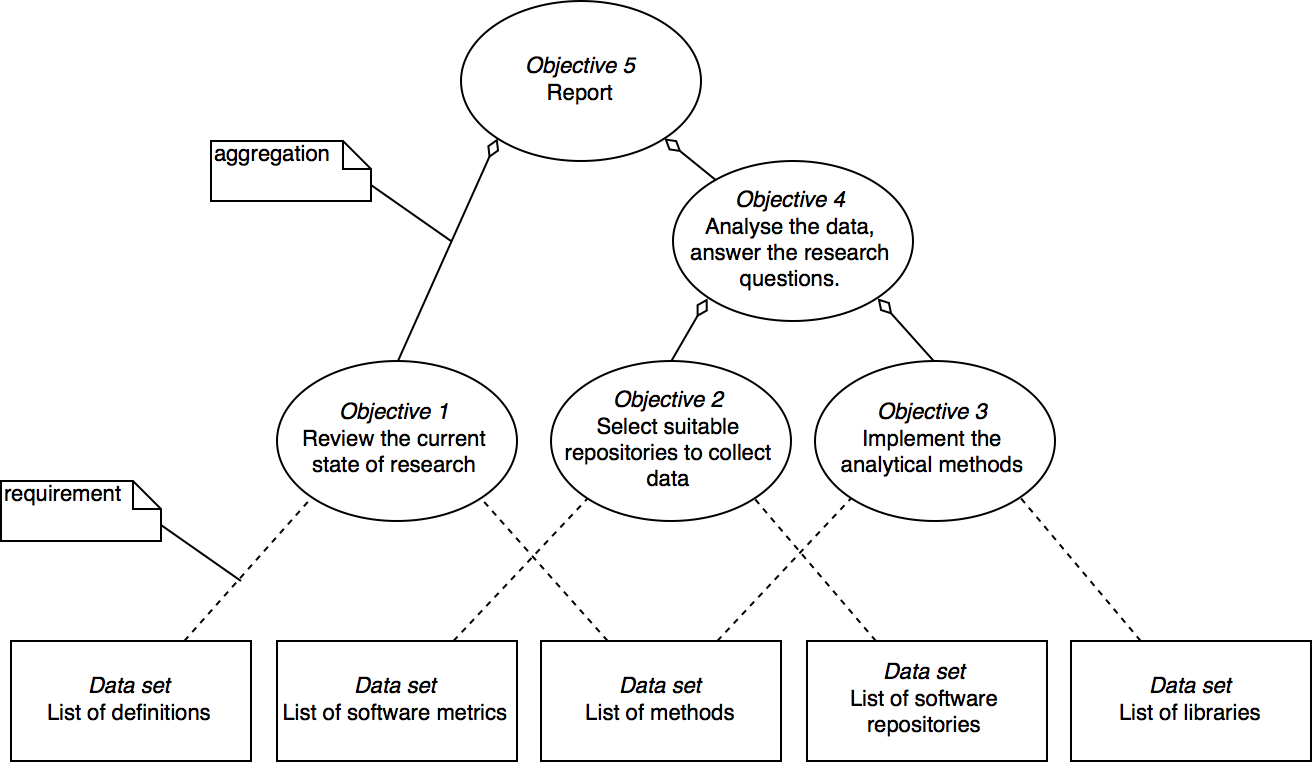
\includegraphics[width=\textwidth]{objectives_questions_and_data.png}
  \caption{Model of objectives and data sets required.}
  \label{fig:objectives}
\end{figure}

\begin{table}[H]
\caption*{Objective 1: Review the current state of research.}
\label{table:objective1} 
\centering
\begin{tabu} to \linewidth{p{5cm} p{5cm} p{5cm}}
\toprule
Task & Dataset & Method \\
\midrule
Attempt a working definition of the terms "fork" and “software evolution”. & A list of definitions. & Literature review \\
\midrule
Select methods from evolutionary biology. & A list of methods. & Literature review \\
\bottomrule
\end{tabu}
\end{table}

\begin{table}[H]
\caption*{Objective 2: Select suitable repositories to collect data.}
\label{table:objective2}
\centering
\begin{tabu} to \linewidth{p{5cm} p{5cm} p{5cm}}
\toprule
Task & Dataset & Method \\
\midrule
Select metrics applicable to software forks. & A list of software metrics. & Literature review \\
\midrule
Select suitable repositories and collect data. & Required or interesting repository characteristics, a list of software metrics. & Literature review \\
\bottomrule
\end{tabu}
\end{table}

\begin{table}[H]
\caption*{Objective 3: Implement the analytical methods.}
\label{table:objective3}
\centering
\begin{tabu} to \linewidth{p{5cm} p{5cm} p{5cm}}
\toprule
Task & Dataset & Method \\
\midrule
Select software libraries. & A list of libraries. & Literature review \\
\midrule
Implement the software & A list of methods. & Documentation review \\
\bottomrule
\end{tabu}
\end{table}

\begin{table}[H]
\caption*{Objective 4: Analyse the data using methods from evolutionary biology. Answer the research questions.}
\label{table:objective4}
\centering
\begin{tabu} to \linewidth{p{5cm} p{5cm} p{5cm}}
\toprule
Task & Dataset & Method \\
\midrule
Answer RQ1 & Data collected (objective 2), set of analytical methods (objective 3) & Estimate phylogenies for each fork case. Analyse. \\
\midrule
Answer RQ2 & Data collected (objective 2), set of analytical methods (objective 3) & Estimate phylogenies, obtained from different character sets. Analyse. \\
\bottomrule
\end{tabu}
\end{table}

\begin{table}[H]
\caption*{Objective 5: Report}
\centering
\begin{tabu} to \linewidth{p{5cm} p{5cm} p{5cm}}
\toprule
Task & Dataset & Method \\
\midrule
Report recommendations for practitioners. & The current state of research (objective 1), the results of the analysis (objective 4) & Compile and present an account. \\
\bottomrule
\end{tabu}
\end{table}

%----------------------------------------------------------------------------------------

\section{Summary of Chapter 2}
The concept of evolution has been used at least since 1980 in a software development context. Moreover, there is an abundant body of work on statistical methods for quantifying and describing biological evolutionary processes. However, although quantitative methods have been used to facilitate project management in different use cases, such as predicting fault-proneness of software, no work was found which applies biological evolutionary techniques to quantify the evolution of software forks. Therefore, primary research was required to answer the research questions specified in paragraph 2.1. In order to carry out this research, 5 objectives were defined: reviewing the current state of research, selecting suitable open source repositories to collect data about forks, porting methods from evolutionary biology to analyse the data acquired from the repositories, and reporting the results for an audience of practitioners.

 
%% Chapter 3

\chapter{Methodology} % Main chapter title

\label{Chapter3} % For referencing the chapter elsewhere, use \ref{Chapter1} 

%----------------------------------------------------------------------------------------

\section{Methods and techniques selected}
In the following sections the term “technique” is used for any procedure that can be boiled down to an algorithm, while the term “method” is used for a coherent combination of techniques.

As illustrated in figure 1.1, and further elaborated in the working definition of “software evolution” in paragraph 1.3, the methods and techniques chosen are applied to a population of software releases. Therefore, the basic entity under scrutiny, the “operational taxonomic unit” \citep{Sokal1986a}, is the “software release”.

\subsection{Data acquisition and encoding techniques}

The choice of techniques for data acquisition is based, with alterations, on the overview of software metrics provided by \citet{Nagappan2008a} reviewed in paragraph 2.2.1. \citet{Nagappan2008a} distinguish between code structure characteristics and organizational characteristics. The following characteristics were used to describe software releases.

\subsubsection{Code structure characteristics}
For the present research, it was assumed that for the study of software evolution, the most relevant code structure characteristic is a measure of code churn, redefined as the amount of change introduced by each release.

\noindent
Code churn was recorded by 2 measurements: 
\begin{itemize}
\item{The presence (or absence) of each file in each specific release.}
\item{a checksum of each file indicating file changes across releases.}
\end{itemize}

\subsubsection{Organizational characteristics}
Software source code is generally developed and stored in a code repository. Code repositories record who edited each file and who committed the change in the repository, thus providing information about the structure of the development team involved in each software release. Team structure characteristics were recorded in three measurements:

\begin{itemize}
\item{\textit{Team composition} was recorded as the presence (or absence) of a team member for each specific release.}
  
\item{\textit{Edit frequency} was recorded as the number of edits by each team member for each release. Editors contribute their knowledge to the code base, so the number of edits indicates how much knowledge is provided by a team.}

\item{\textit{Code ownership} was recorded as the number of commits by each team member for each release. Committers control which edits make it into the code base, so the number of commits indicates how much a release is owned by a team.}
\end{itemize}

\begin{table}[H]
\caption{Summary of characteristics and their data types}
\label{table:characteristics} 
\centering
\begin{tabu} to \linewidth{p{5cm} p{5cm} p{5cm}}
  \toprule
  Characteristic & Domain & Data type \\
  \midrule
  Presence (or absence) of a file in a release &
  One measurement for each version of a file in a release &
  Boolean \\
  \midrule
  File changes (checksums) &
  One measurement for each version of a file in a release &
  categorical \\
  \midrule
  Team composition &
  One measurement for each team member contributing to a release &
  Boolean \\
  \midrule
  Edit frequency &
  One measurement for each team member contributing to a release &
  integer \\
  \midrule
  Code ownership &
  One measurement for each team member contributing to a release &
  integer \\
\bottomrule
\end{tabu}
\end{table}

\subsection{Techniques for computing the distance matrix}
As discussed in the review of literature on evolutionary techniques (2.2.3), “distance matrix methods”, i.e. evolutionary techniques that use a matrix of pairwise dissimilarity between entities to estimate a classification \citep{FelsensteinJ.andFelenstein2004a} offer an approach that produces accurate results and performs well on large data sets.

The distance matrix is computed on the base of the measurements obtained using the techniques described in paragraph 3.1.1. The result is a matrix with one column and one row for each software release, were each cell contains a measure of the pairwise dissimilarity between the corresponding two releases. As the measurements used are of different data types (table \ref{table:characteristics}), a technique that can calculate the distance matrix by combining measurements of mixed data types is required. The Gower distance provided by the R-package “StatMatch” provides such an algorithm \citep{DOrazio2016}.

\subsection{Estimating the phylogeny of releases}
Having computed a distance matrix using the techniques described in paragraph 3.1.2, the next step is to estimate a phylogenetic tree that represents the relationships between the software releases studied. The choice of techniques for estimating trees is based on the reference provided by \citet{Paradis2011}, as discussed in 2.2.2. Commonly used techniques for estimating trees include:

\begin{description}
\dt{Average linkage (UPGMA)} \dd{UPGMA is a method that generates a tree based on the degree of similarity between entities \citep{Sneath1962a}, but does not imply a descent from a common ancestor. Therefore it is a “phenetic” method, i.e. the result is a hierarchical clustering of the entities under scrutiny, based on their characteristics \citep{Rohlf2013a}.}
\dt{Neighbour-Joining (NJ)} \dd{NJ is a “cladistic” method, i.e. it assumes a descent from common ancestry and seeks the tree with the fewest possible evolutionary changes, i.e. the tree with the “maximum parsimony” \citep{Rohlf2013a}. As working on trees is a complex problem, a heuristic is used to make the search more efficient: NJ seeks the tree with the shortest total branch length, i.e. the tree with the least amount of changes, and accomplishes this by iteratively re-computing the dissimilarity matrix \citep{Saitou1987a}.}
\dt{Minimum Evolution (ME)} \dd{ME is similar to NJ in its aims, but it seeks the shortest tree by applying a different heuristic: seeking the tree with the shortest overall branch length by rearranging the topology of the tree \citep{Desper2005a}.}
\end{description}

\subsection{Cophenetic distance matrix}
The cophenetic distance is the distance at which two tips of a tree combine into a single branch \citep[p.1275]{RDevelopmentCoreTeam2008a}. A cophenetic distance matrix can be calculated for the pairwise distances as represented in the tree. Cophenetic distance matrices were used here for two purposes:

\begin{description}
\dt{As a measure of accuracy} \dd{The correlation between the distance matrix (obtained from measurements) and the cophenetic distance matrix (obtained from the tree) is a way of telling how well the tree represents the data and can be used to assess the accuracy of the phylogenetic methods \citep{Sokal1986a}.}

\dt{As input for further analysis} \dd{As the cophenetic distance matrix represents the tree, it can be used as input for statistical analysis. Cophenetic matrices were used to answer the research questions, as detailed in the following paragraph.}
\end{description}

% ----------------------------------------------------------------------------------------

\section{Justification}
The practical problem (2.1) was tackled through two research questions. These research questions were answered by reformulating them as statistical hypotheses based on the trees obtained by applying the methods and techniques selected. Cophenetic distance matrices (3.1.4) were instrumental in defining these statistical hypotheses, as cophenetic distance matrices represent the trees in a way that can be used as input for statistical analysis.

\subsection{RQ1}
Research Question 1 sought to determine a threshold beyond which two diverging branches will be more likely to fork than to merge. This result was expected to provide guidance as to the preferred strategy to follow when part of the team is getting off on its own by answering the question: is a merge still practicable or is a fork unavoidable?

\definition{Null hypothesis}{The null hypothesis is that branches and forks are indistinguishable by measuring the pairwise distance between releases.}

\definition{Alternative hypothesis}{The alternative hypothesis is that a branch can be told from a fork by measuring the pairwise distance between releases.}

\noindent
These hypotheses can be translated into statistical hypotheses by examining the cophenetic distance matrix obtained from the estimated phylogenetic tree.

\definition{Statistical null hypothesis}{The statistical null hypothesis is that the mean cophenetic distances between releases on the same branch and on different forks are not significantly different.}

\definition{Alternative statistical hypothesis}{The alternative statistical hypothesis is that the mean cophenetic distance between a pair of releases is significantly different (p < 0.05) depending on whether the releases are on different forks or on the same branch.}

\subsection{RQ2}
Research Question 2 sought to determine whether the outcome of a fork can be predicted through phylogenetic methods. The predicted outcome was expected to fall into one of three categories: cooperation, competition or discontinuation. This result would provide guidance as to which outcome is to be expected in the future of the fork and which strategy is more suitable to attain the project's goals. 

The expected outcome was that two distinct but cooperating teams would produce a code base with many similarities, while two competing teams would produce clearly distinct code bases. The proposed method for answering this question is to use the same approach as in RQ1, but applying it to the two data sets obtained from code measurements and team measurements, thus estimating a “code-base tree” and a “team tree” for each fork. 

\definition{Null hypothesis}{The null hypothesis is that forks with different outcomes are indistinguishable based on code and organizational measurements.}

\definition{Alternative hypothesis}{The alternative hypothesis is that the outcome of a fork can be predicted by measuring the pairwise distances between releases, based on separate code and organizational data sets.}

\noindent
These hypotheses can be translated into statistical hypotheses by calculating the variance of the cophenetic distances between trees of forks obtained from code measurements and trees constructed from team measurements.

\definition{Statistical null hypothesis}{The statistical null hypothesis is that the mean distance between forks with different outcomes are not significantly heterogeneous with regard to the outcome of the fork.}

\definition{Alternative statistical hypothesis}{The alternative statistical hypothesis is that the mean distance between forks with different outcomes are significantly heterogeneous with regard to the outcome of the fork.}

%----------------------------------------------------------------------------------------
\section{Research procedures}
The research questions are examined by applying the activities detailed in figure \ref{fig:methods}.

\begin{figure}[H]
  \centering
  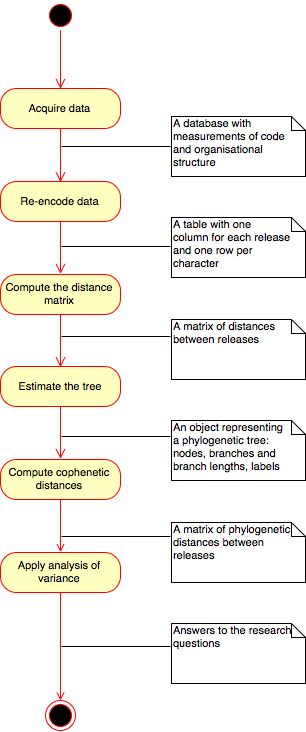
\includegraphics[width=0.5\textwidth]{methods.png}
  \caption{Activity diagram of the steps necessary for estimating phylogenetic relationships using distance-based methods, as implemented for the present research.}
  \label{fig:methods}
\end{figure}

\subsection{Data acquisition and re-encoding}
Data was acquired from selected open source repositories. The choice of software projects to study was guided by the comprehensive review of forks provided by \citet{Robles2012a}. Forks are per definition only possible in an open source context, therefore any conclusions apply in this context only. Additionally, the choice of projects was limited by the availability of a complete release history of the project, at least as far back as the moment in time were the fork happened.

As forking is a process at the crossroads between technical evolution and organizational evolution (as per the definition in paragraph 1.3), the data acquisition techniques were chosen to cover technical and organizational aspects of projects.

Data has to be re-encoded in order to be processable. This process is explained in detail in paragraph 4.1.2. Guidelines for re-encoding characters can be found in \citet{Sokal1986a}.

\subsection{Distance matrices}
As explained in paragraph 3.1.2, the chosen methods for answering the research questions are all part of the “distance matrix” family of phylogenetic methods. As shown in figure 3.1, a matrix of the pairwise dissimilarity between the releases of the chosen fork has to be computed. Several techniques are available to compute a distance matrix: computing Euclidean, or “Manhattan” distances are commonly used \citep{Felsenstein1982a}. However, these techniques are limited to processing numerical and Boolean data respectively. As the acquired data is of various data types (Boolean, categorical, numerical, see table \ref{table:characteristics}) the chosen method is required to process different data types. Only the “Gower” technique \citep{DOrazio2016} satisfies this requirement. However, the Gower technique is limited in that matrix rows with missing values do not contribute to the result, therefore, part of the data acquired was discarded before processing.

Table 3.2 shows an example distance matrix, constructed by subsampling the data collected for the Mysql / MariaDB fork (see 4.1 for details). Ten branches and thousand measurement characters were selected at random (the original data set has 107 branches and 56 648 measurement characters).

\subsection{Phylogenetic trees and cophenetic distances}
The proposed methods for answering the research questions involve constructing phylogenetic trees by applying the methods described in 3.1.3.

Figure \ref{fig:sample_tree} shows an example tree constructed using the subsample of the data presented in table 3.2. The Neighbour-Joining algorithm \citep{Saitou1987a} was used to estimate the tree.

\begin{figure}[H]
  \centering
  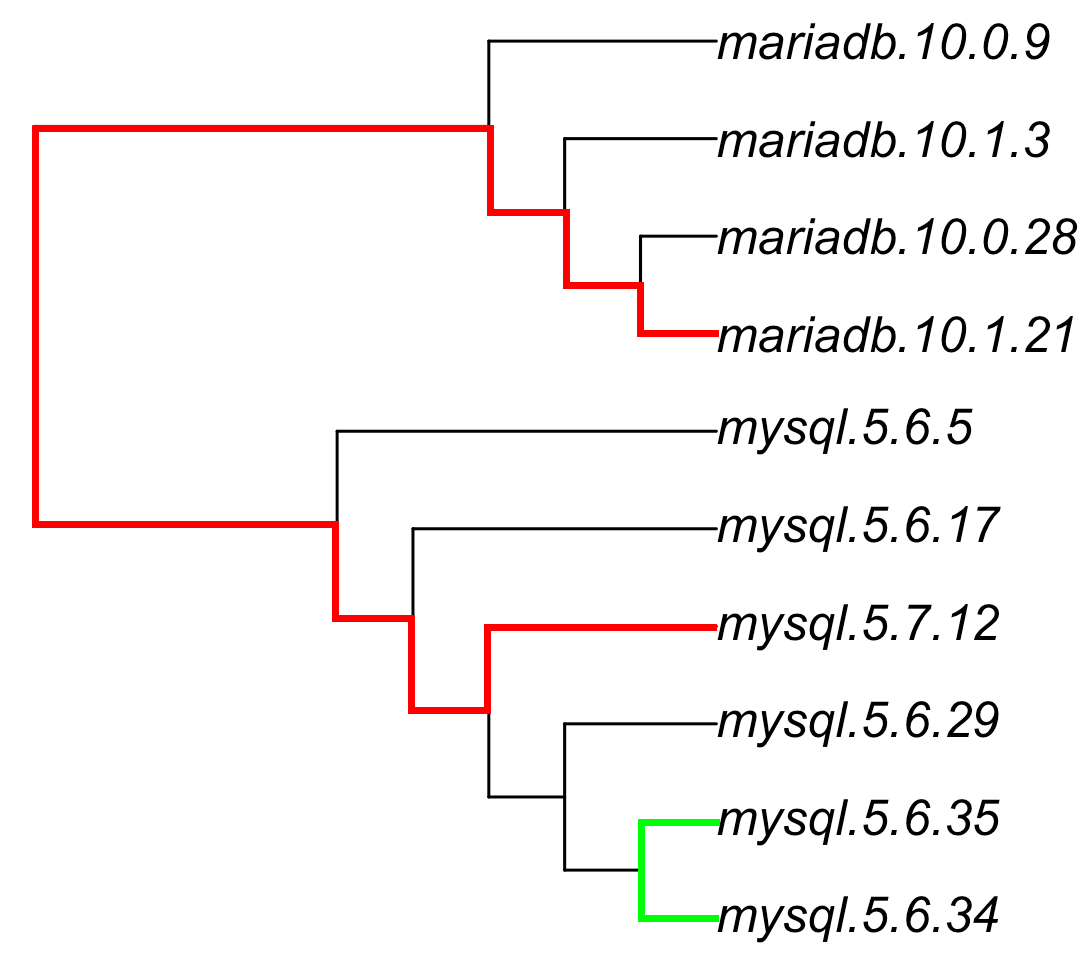
\includegraphics[width=0.5\textwidth]{mysql_sample_tree.png}
  \caption{An example tree obtained by applying the NJ method to the data in table 3, showing the longest (red) and shortest (green) distances between tips of the tree.}
  \label{fig:sample_tree}
\end{figure}

The next step is to calculate the cophenetic distances between the tips of the trees. Figure 3.2 illustrates this: the green line represents the shortest path between two tips in the example; the red line represents the longest path between two tips.

Table 3.3 shows an example cophenetic matrix. Please note that the cophenetic matrix is calculated from the tree, so the method used to estimate the tree has an effect on the cophenetic matrix. Conversely, the correlation between the distance matrix and the cophenetic matrix can be used as a measure of how accurately the tree represents the distance matrix.

The distance matrix can be shaded to show the degree of dissimilarity between releases, and the matrix can then be rearranged into clusters of the same shade. This representation was introduced by \citet{Sneath1962a} and used to discover species and genus in the data. Table 3.4 shows that in the example data, MySQL releases are close to each other, while MySQL 5.7.12 and all releases of MariaDB are the most distant from each other (light-shaded cells in the bottom row).

\subsection{Analysis of variance}
As detailed in 3.2.1, answering RQ1 requires computing a matrix of the cophenetic distances between releases and estimating if these distances correlate to forks and branches. Figure \ref{fig:example_boxplot} shows a box plot of the cophenetic distances in the example data. The plot shows that distances between tips inside either project (“Branches”) are statistically smaller than the distances between tips on different forks (“Forks”).

\begin{figure}[H]
  \centering
  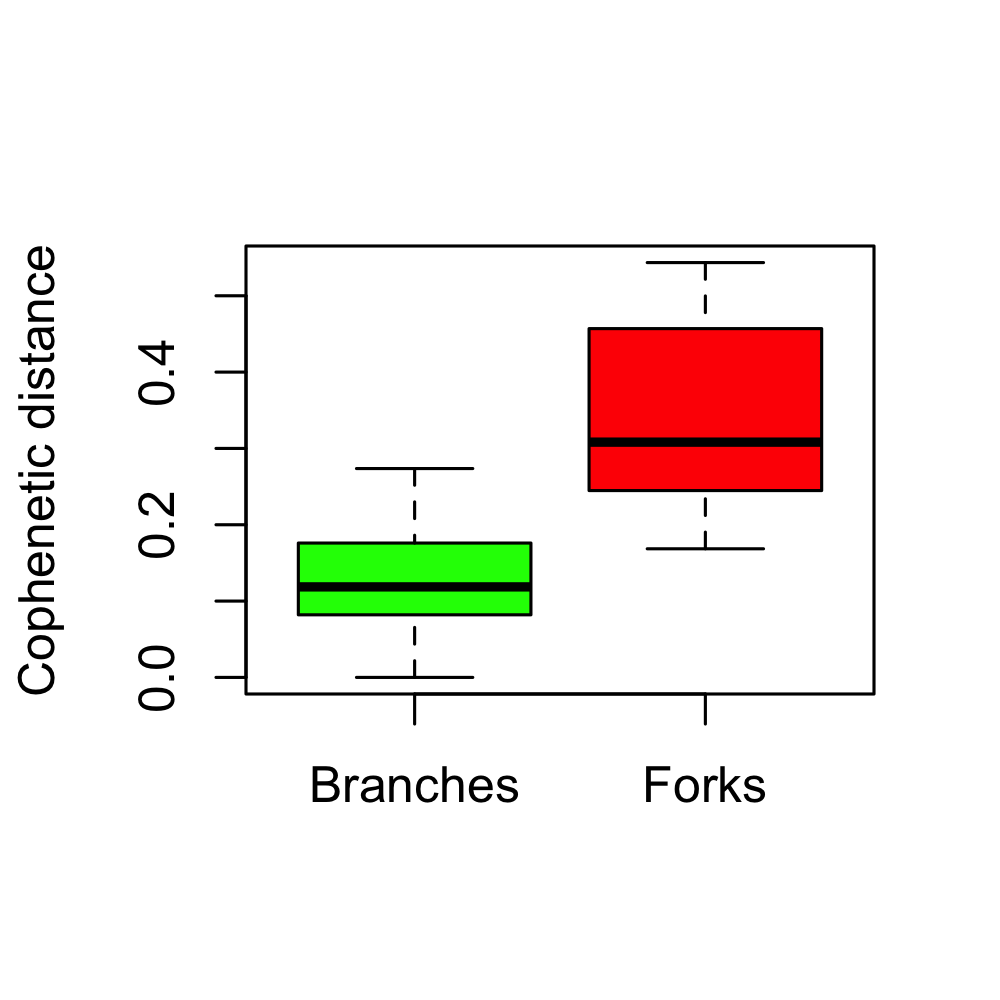
\includegraphics[width=0.5\textwidth]{example_boxplot.png}
  \caption{A box plot of the cophenetic distances of branches and forks in the example data.}
  \label{fig:example_boxplot}
\end{figure}

According to \citet{McDonald2014b}, choosing a method for statistical analysis is primarily guided by the kind and number of variables required to test the hypothesis. The cophenetic distance is a measurement variable, and whether the pairwise distance between releases corresponds to a “fork” or “branch” is a nominal variable. \citet{McDonald2014b} lists two methods for testing a hypothesis based on one measurement and one nominal variable: “student's t-test” and “analysis of variance” (ANOVA).

The method proposed for answering RQ2 (paragraph 3.2.2) requires examining projects with different outcomes and computing two cophenetic distance matrices for each project: one for the tree obtained from team measurements, and a second one for the tree obtained from code measurements. Having computed these matrices, the next step is to estimate if these distances correlate with different project outcomes. The cophenetic distance is a measurement variable, the data set used (“team measurements” or “code measurements”) is a nominal variable and the outcome of the project (“cooperation”, “competition” or “discontinuation of a branch”) is a second nominal variable. \citet{McDonald2014b} recommends applying a two-way ANOVA for testing a hypothesis based on one measurement and two nominal variables.

Consequently, RQ1 and RQ2 can be answered by applying analysis of variance (ANOVA), albeit with different number of nominal variables. ANOVA assumes that the data is normally distributed (fits the Gaussian “bell curve”) and that that the standard deviation is the same for the data sets examined, otherwise false positives may result \citep[p.147]{McDonald2014b}. As the raw data obtained from the repositories did not meet these assumptions, the data had to be transformed to fit the assumptions prior to the analysis.

%----------------------------------------------------------------------------------------
\section{Ethical considerations}
All data analysed for this research is freely available under an open source license, therefore no intellectual property rights were disregarded during the acquisition of the data. 

Some of the forks studied were a consequence of disagreements between development teams. Care was applied during the analysis not to take sides for any particular team; however, to thwart any bias ensuing from the reputation of well-known actors in the industry, all names of developers were anonymized prior to being stored locally.

Although I do participate in open source software development, I am not involved in any of the projects examined for this research.
%----------------------------------------------------------------------------------------
\section{Summary of Chapter 3}
Character measurement techniques applicable to software code bases and to software producing organizations were selected from literature. Suitable techniques to study the evolution of software were chosen from the corpus of biological techniques for estimating phylogenetic trees. The two research questions were specified in terms of hypotheses, null hypotheses and their corresponding statistical hypotheses. The steps required by the research were worked out and each step was illustrated with an example drawn from a subset of the data. Finally, analysis techniques suitable to answer the research questions were selected, based on the type and number of independent variables required by the analysis.



%% Chapter 4

\chapter{Analysis and interpretation} % Main chapter title

\label{Chapter4} % For referencing the chapter elsewhere, use \ref{Chapter1} 

%----------------------------------------------------------------------------------------

\section{Summary of data collected}
In order to answer the research questions (2.1), three cases of forks with different outcomes were selected. Forking reasons and outcomes are characterized here using the terminology introduced by \citet{Robles2012a}.

\begin{description}
\dt{MySQL server / MariaDB server}
\dd{The open source database server MySQL was purchased by Sun Inc. in 2008, resulting in the departure of the original chief engineer (on good terms) to form his own company, MariaDB \citep{Widenius2009}. Subsequently, Sun was acquired by Oracle. Oracle’s attempt to highjack the project \citep{Nyman2013a} led to a full-fledged fork in 2012 \citep{Widenius2012}.}

\dt{Linux kernel / Android kernel}
\dd{In 2005, Google Inc. bought Android, then a start-up developing a Linux-based operating system for cellular phones, in order to expand its search service to the mobile market \citep{Elgin2005}. The Linux community and Google have been cooperating on the core system, while Google continues to develop device-specific extensions to the core under a shared open source licensing regime \citep{Vaughan-Nichols2011}.}

\dt{Apache OpenOffice / LibreOffice}
\dd{Development of the OpenOffice suite of office applications began in 2000, in a company owned by Sun Microsystems; following the acquisition of Sun by Oracle, OpenOffice was forked into LibreOffice by its developers in 2010; as OpenOffice lost momentum, Oracle donated the project to the Apache foundation in 2011 \citep{Gamalielsson2014b}.}
\end{description}

\subsection{Data acquisition}
In order to make the data easier to process, a database was populated with data obtained from the projects' repositories (Appendix 1). A script was written in Python to collect the data from the software repositories, and a second script to compute the metrics. The scripts were written applying test-driven-development to ensure their correctness and maintainability. Data collection was automated, so the process is repeatable.

Team members were identified by their login name, publicly available through the repositories’ logs. Login names were replaced by non-reversible unique hashes prior to being stored in a local database (in line with ethical considerations in paragraph 3.4).

The raw data as obtained from the repositories and stored in the local database is summarized in table 4.4.

\subsection{Exporting and recoding the data for analysis}
The measurements obtained from the data were exported in a format suitable for analysis: a spreadsheet where columns represent releases and rows represent measured characteristics.

\begin{itemize}
\item{For code characteristics, one column for each release and 2 rows for each file: "presence/absence" and "checksum".}
\item{For team characteristics, one column for each release and 3 rows for each contributor: "presence/absence" in team, "edits count" and "commits count".
A Python script was written to export the data. The script handles re-encoding and cleaning-up the data, discussed below.}
\end{itemize}

\subsubsection{Re-encoding}
Binary characters, e.g. presence/absence of a file in a branch, were encoded as a row of Boolean values. Count characters were encoded as integers. Measurement characters, e.g. checksums of files, were recoded into classes: if a file is the same for all branches, there was only one class, if a file changes in all branches, there were as many classes as branches and so on (see table 3.1 for an overview of the data types used).

\subsubsection{Cleaning-up}
The data had to be cleaned-up before processing: only rows which are complete could be used for calculating the distance matrix, e.g. if a file is missing in a release, its corresponding “checksum” row had to be discarded. Cleaned-up data represents between 53 and 64 \% of the raw data, depending on the fork (table 4.5).

\subsection{Applying phylogenetic methods}
Distance matrices were computed and phylogenetic trees were estimated for each fork case studied. The software was written using the R language for statistical computing \citep{RDevelopmentCoreTeam2008a}. The classes implemented are wrappers for the R functions provided by packages for general and biological statistics. 

The software implemented for the research is documented in the class diagram in Appendix 2.

\begin{itemize}
\item{Distance matrices were calculated using the function “gower” provided by the R-package “StatMatch” \citep{DOrazio2016}.}

\item{The UPGMA technique for computing taxonomic trees (3.1.3) was implemented using the function ”hclust” with the agglomeration method “UPGMA” provided by the R-package “Stats” \citep[p.1355]{RDevelopmentCoreTeam2008a}.}

\item{The Neighbour-Joining and Minimum Evolution techniques (3.1.3) were implemented using the functions “nj” and “fastme.bal” provided by the R-package “Ape” \citep{Paradis2004a}.}
\end{itemize}

\subsection{Cophenetic distances}
Answering the research questions involves calculating a cophenetic distance matrix for each tree. Cophenetic distances were calculated using the function “cophenetic” provided by the R-package “Stats” \citep[p.1275]{RDevelopmentCoreTeam2008a}.

%----------------------------------------------------------------------------------------

\section{Data analysis}

\subsection{Answering RQ1}
Answering RQ1 (see paragraph 2.1) requires calculating the distance between software releases and estimating if these distances correlate to forks and branches. The expected outcome is that forks will always differ more than branches, independently of the outcome of the project.

\subsubsection{Choice of statistical method for analysis}
Whether a pair of releases represents a fork or a branch is a nominal variable with two possible values (“fork” or “branch”) and the pairwise cophenetic distance between releases is a measurement variable. A suitable test for these types of variables is a one-way analysis of variance (ANOVA) with two categories \citep{McDonald2014b}. The result should be repeatable for each case described in 4.1. The R-package “Stats” provides methods for computing variance \citep[p.1211]{RDevelopmentCoreTeam2008a}.

\subsubsection{Checking assumptions for RQ1}

\definition{Assumption 1: Accuracy}{Methods for computing trees from distance matrices are assumed to produce trees that represent the distance matrix accurately.}

\noindent
The three methods chosen in 3.1.3 (UPGMA, NJ, ME) were applied, and the correlation between the distance matrix and the cophenetic matrix obtained from each tree was used as a measure of how accurately the trees represent the distance matrix \citep{Rohlf2013a}. Correlations (Pearson's Chi-squared test) were calculated for each fork (table 4.6). The Neighbour-Joining method was found to produce the best correlation for the 3 data sets considered (correlation > 0.991086), UPGMA is second (correlation > 0.823779) and ME is the most inaccurate method (correlation > 0.512404).

\definition{Assumption 2: Normality}{ANOVA assumes that the data is normally distributed (fits the Gaussian “bell curve”) and that the standard deviation is the same for the data sets examined. Performing an ANOVA on data sets that are not normally distributed increases the chance of false positives \citep[p.147]{McDonald2014b}.}

\noindent
As can be seen in figure \ref{fig:rq1_distributions}, the data is not normally distributed. An accepted remedy for this situation is to transform the data to make it fit the assumption of normality better: common transformations are to apply logarithm or square root transformations to the data \citep[p.141]{McDonald2014b}. The histograms (\ref{fig:rq1_distributions}) show that the distribution of the square root of distances (in figure \ref{fig:rq1_distributions}, bottom row) better fits the normal distribution.

\begin{figure}[H]
  \centering
  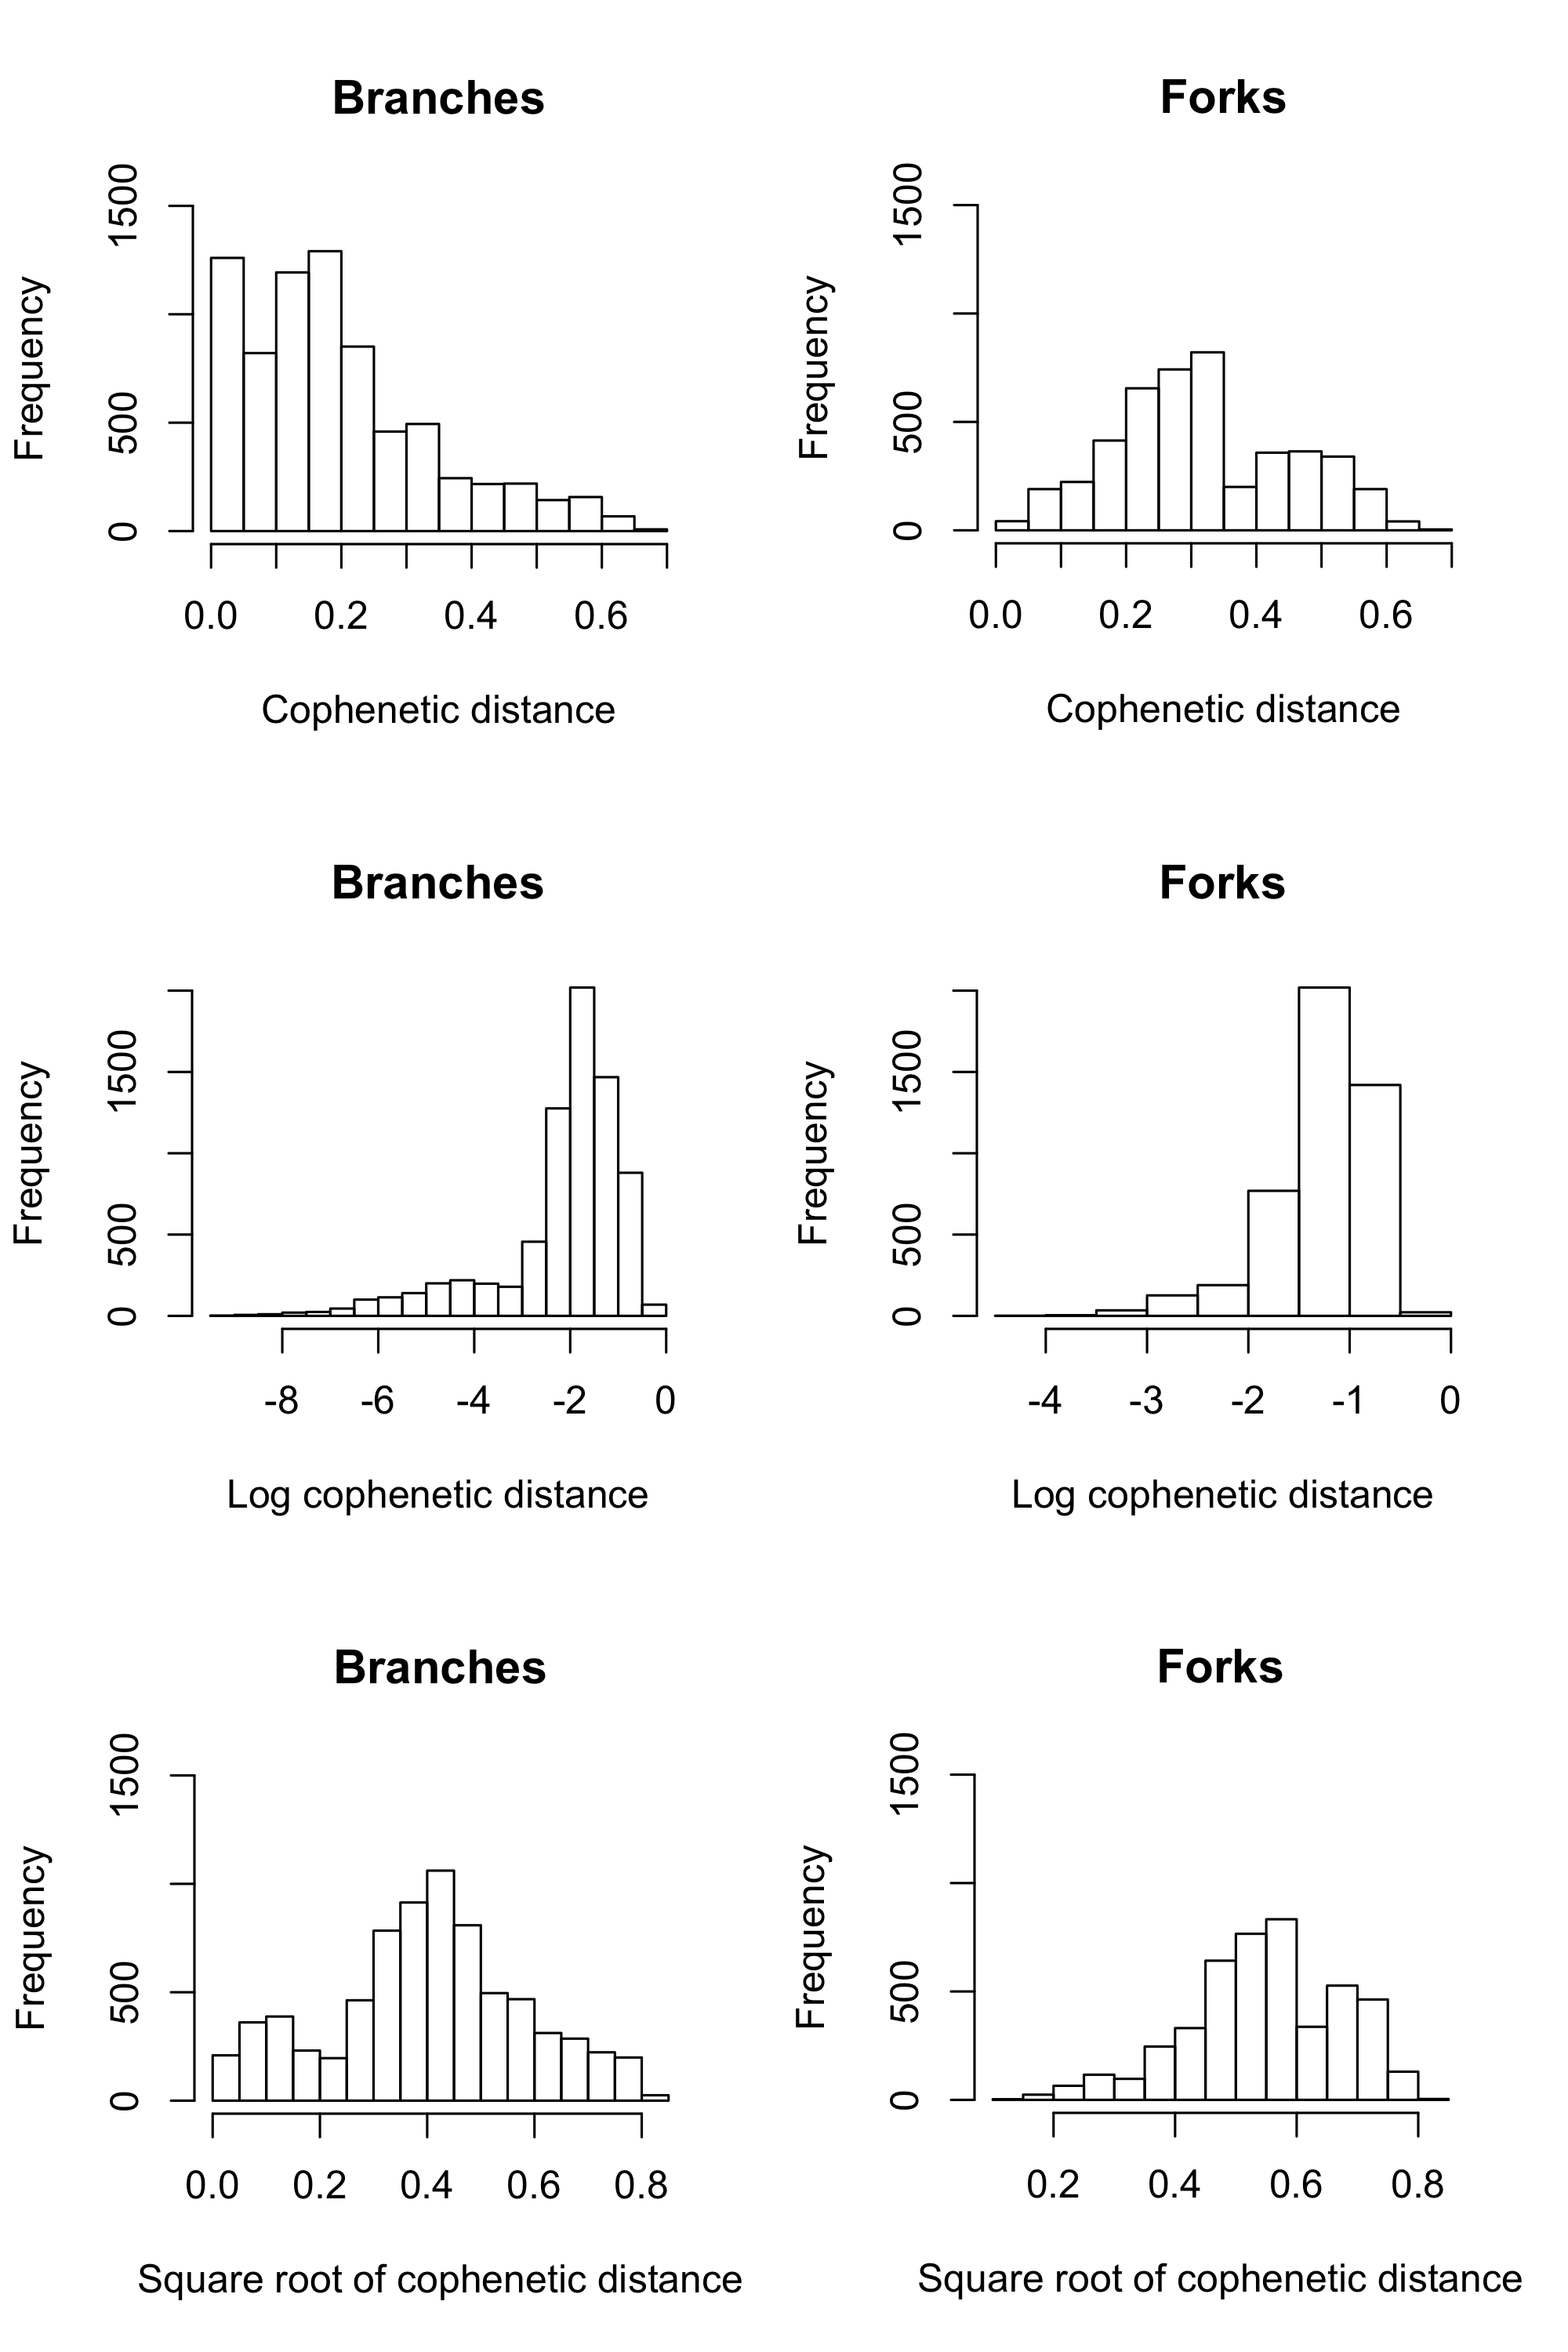
\includegraphics[width=\textwidth]{rq1_distributions.png}
  \caption{Histograms illustrating the distribution of the cophenetic distances, obtained by applying the NJ method to branches and forks of all projects considered. The top row shows untransformed distances, the middle row shows the base-10 logarithm of the distances and the bottom row the square root of the distances.}
  \label{fig:rq1_distributions}
\end{figure}

\definition{Assumption 3: Homoscedasticity}{ANOVA assumes that the standard deviation of the data is the same for the data sets considered (the data is “homoscedastic” or else it is “heteroscedastic”). Performing an ANOVA on heteroscedastic data sets increases the chance of false positives \citep[p.147]{McDonald2014b}.}

\noindent
Table 4.7 shows that the cophenetic distances obtained by applying the NJ method to the square root transformed data set is homoscedastic within reason, i.e. the ratio between the standard deviation of branches and forks is relatively small (0,0020998 /  0,0018566 = 1,1309758). Therefore, performing an ANOVA on the square root transformed data should minimize the chance of false positives.

\subsubsection{One-way analysis of variance (ANOVA)}
The analysis involved the following steps:

\begin{enumerate}
\item{Distance matrices were computed from the data acquired for each project, using the Gower technique, as data is of various types (Boolean, integer, categorical, see table 3.1).}

\item{Trees were estimated from these distance matrices by applying the Neighbour-Joining (NJ) method, which seems to represent the distance matrix in an accurate way (as discussed under “checking assumptions for RQ1”).}
  
\item{A cophenetic distance matrix was obtained from each tree (the measurement variable).}
  
\item{Cophenetic distances were aggregated into “branches” and “forks” (the nominal variable).}

\item{One-way ANOVA was performed on the square-root of the cophenetic distances.}
\end{enumerate}

The analysis of the square root transformed data with one-way ANOVA (table 4.8) show that the nominal variable “release type” (i.e. “branches” or “forks”) has significant influence on the cophenetic distance between releases (p < 2e-16). Therefore the null hypothesis can be rejected.

This result is visualised in the plot in figure \ref{fig:rq1_all}: The mean cophenetic distance between releases on different forks is larger than the mean distance between releases on different branches, using data from the three projects considered.

\begin{figure}[H]
  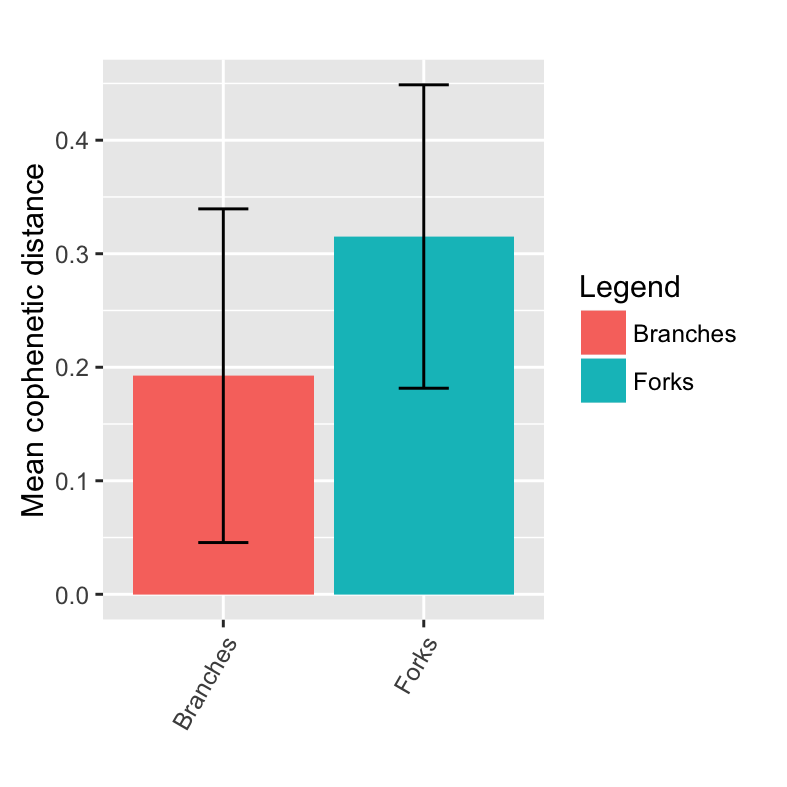
\includegraphics[width=\textwidth]{RQ1_all.png}
  \caption{Plot of the mean cophenetic distances between releases and their standard deviation for all fork cases combined.}
  \label{fig:rq1_all}
\end{figure}

\subsection{Answering RQ2}
Answering RQ2 (see paragraph 2.1) requires examining the phylogenetic trees of forks with different outcomes (competition, cooperation, discontinuation of a branch) and seeking a correlation between the outcome of the fork and the topology of the tree.

The proposed method for answering this question is to use the same approach as in RQ1, but applying it to the two data sets obtained from code measurements and team measurements, thus estimating a “code-base tree” and a “team tree” for each fork. As explained in paragraph 3.2.2, the rationale for this approach is that two distinct but cooperating teams are expected to produce a code base with many similarities, while two competing teams will produce clearly distinct code bases. Therefore answering RQ2 required treating organizational and code measurements separately. Furthermore, as different organizations and code bases were compared, measurements representing the pairwise differences between releases within the same organization, i.e. “branches”, were discarded, and only “fork” measurements were analysed.

\subsubsection{Choice of statistical method for analysis}
The outcome of a fork is a nominal variable with three categories (“competition”, “cooperation”, “discontinuation”), the data-set used to construct the tree is a second nominal variable with two categories (“code” and “team”) and the cophenetic distance between releases on different forks is a measurement variable. The null hypothesis for RQ2 is that the mean cophenetic distance is not significantly different for the “outcome” categories considered. Rejecting the null hypothesis would provide evidence that the outcome of a fork can be predicted. A suitable test for this case is a two-way ANOVA \citep{McDonald2014b}, where the measurement variable is the cophenetic distance between releases on different forks, and the two nominal variables are the outcome and the data-set used.

\subsubsection{Checking assumptions for RQ2}
The assumptions of accuracy, normality and homoscedasticity apply to a two-way ANOVA as they do to a one-way ANOVA \citep[p.176]{McDonald2014b} but have to be checked against code measurements and team measurements to answer RQ2.

\definition{Assumption 1: Accuracy}{}

\noindent
As for RQ1, the three methods chosen in 3.1.3 (UPGMA, NJ, ME) were applied, and the correlation between the distance matrix and the cophenetic matrix obtained from each tree was used as a measure of how accurately the trees represent the distance matrix \citep{Rohlf2013a}. Correlations were calculated for each data set and fork (table 4.9). The Neighbour-Joining method was found to produce the best correlation (correlation > 0.9911107), UPGMA is second (correlation > 0.8251281) and ME was the most inaccurate method (correlation > 0.0778508).

\definition{Assumption 2: Normality}{A two-way ANOVA assumes, as a one-way ANOVA does, that the data is normally distributed.}

\noindent
Performing a two-way ANOVA on data sets that are not normally distributed increases the chance of false positives \citep[p.176]{McDonald2014b}.

Figure \ref{fig:rq2_distributions}, illustrates the distribution of the cophenetic distances, obtained by applying the NJ method to data sets of code and team measurements separately. As explained in paragraph 4.2.2, only forks are considered for RQ2. The top row in figure \ref{fig:rq2_distributions} shows untransformed distances, the middle row shows the base-10 logarithm of the distances and the bottom row the square root of the distances. The histograms show that the distribution of the square root of distances (\ref{fig:rq2_distributions}, bottom row) better fits the normal distribution.

\begin{figure}[H]
  \centering
  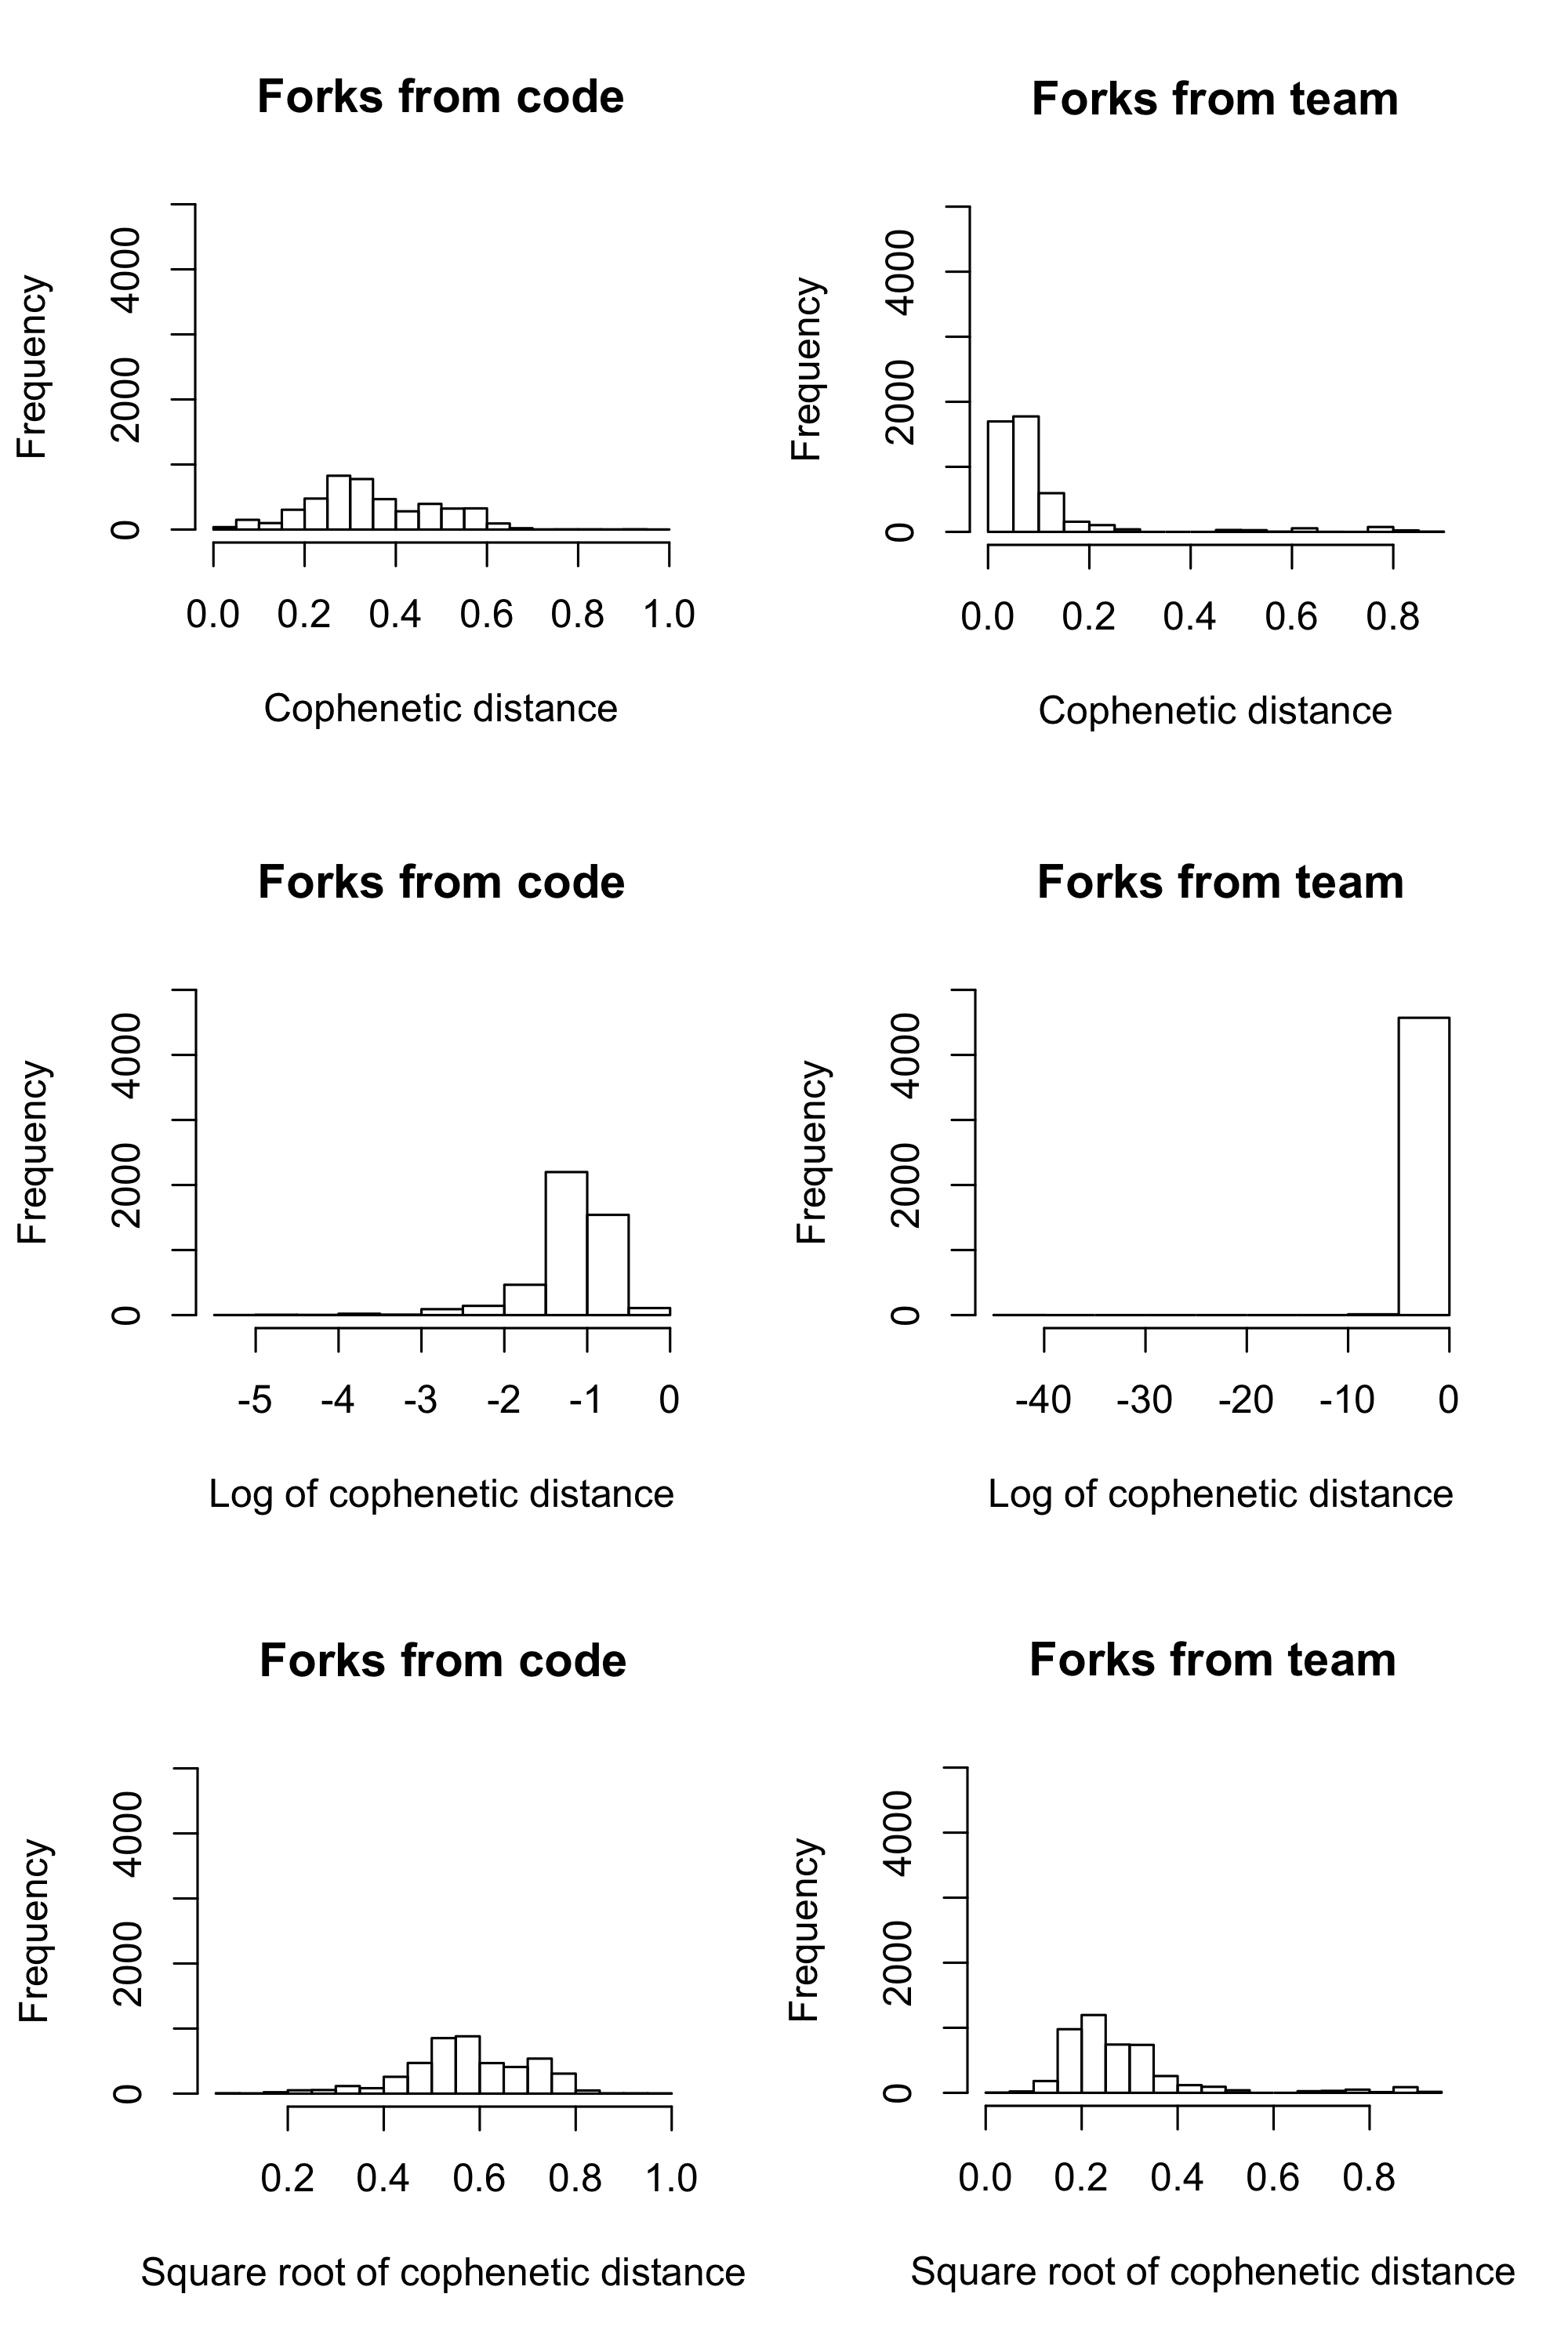
\includegraphics[width=\textwidth]{rq2_distributions.png}
  \caption{Histograms illustrating the distribution of the cophenetic distances: top row untransformed distances, middle row base-10 logarithm of the distances and bottom row square root of the distances.}
  \label{fig:rq2_distributions}
\end{figure}


\definition{Assumption 3: Homoscedasticity}{Two-way ANOVA assumes that the standard deviation of the data is the same for the data sets considered; performing a two-way ANOVA on heteroscedastic data sets increases the chance of false positives \citep[p.176]{McDonald2014b}.}

\noindent
Table 4.10 shows that the square root transformed data set is homoscedastic within reason, i.e. the ratio between the standard deviation of fork distances from team and code data is relatively small (0.1435011 / 0.1258846 = 1.1399417). Therefore, performing a two-way ANOVA on the square root transformed data should minimize the chance of false positives.

\subsubsection{Two-way analysis of variance}
The analysis involves the following steps:

\begin{enumerate}
\item{Distance matrices were computed from the data acquired for each fork, using the Gower technique, as the data is of various types (Boolean, integer, categorical, see table 3.1). Data obtained from code and team measurements was treated separately.}
\item{Trees were estimated from these distance matrices by applying the Neighbour-Joining (NJ) method, which was found to represent the distance matrix in an accurate way (as discussed under “checking assumptions for RQ2”).}
\item{A cophenetic distance matrix was obtained for the “code” and “team” data sets (the first nominal variable) for each project outcome, i.e. “collaboration”, “competition” and “discontinued fork” (the second nominal variable).}
\item{The pairwise distances between releases on the same branch were discarded, leaving a matrix of pairwise distances between forks.}
\item{Two-way ANOVA was performed on the square-root of the cophenetic distances (the measurement variable), as the square root transformed data is closer to a normal distribution than the raw data and is reasonably homoscedastic (as discussed under “checking assumptions for RQ2”).}
\end{enumerate}

The analysis of the square root transformed data with two-way ANOVA (table 4.11) showed that the nominal variable “dataset” (i.e. “code” or “team”) has significant influence on the cophenetic distance between releases (p < 2e-16), but the nominal variable “outcome” (i.e. “cooperation”, “competition” or “discontinued branch”) does not (p = 0.7808). Therefore, the null hypothesis cannot be rejected.

% ----------------------------------------------------------------------------------------

\section{Interpretation in relation to the objectives}
This research set itself five objectives: review the current state of research, select suitable repositories to collect data, implement the analytical methods, analyse the data using methods from evolutionary biology, report for an audience of practitioners.

\subsection{Objective 1: Review the current state of research}
The first objective, to review the current state of research, showed that many similarities exist between biological and software evolution: biological concepts such as “ecosystem”, “lineage” and “evolution” have been used effectively to describe biological and software systems. There are however significant gaps, e.g. what constitutes a “gene” in a software context remains unclear. Furthermore, the literature research emphasizes that the study of forking is a lively research area.

However, to the best of my knowledge, there is very little work on transferring methods from evolutionary biology, in particular phylogenetic methods, to computer science. Therefore, primary research was required to assess whether the chosen methods are applicable to the study of software evolution in general and forking in particular.

\subsection{Objective 2:  Select suitable repositories to collect data}
The second objective, to select suitable repositories to collect data, showed that many open source repositories are accessible and can be mined for data on their release history and team composition. The source code had to be available online and additionally, the project's history back to the moment in time when the fork took place had to be available as well. Suitable projects were found and three were selected for analysis. The quantity of data collected justified the use of a database to store the data.

\subsection{Objective 3: Implement the analytical methods}
The third objective, to implement the analytical methods, was facilitated by the many libraries available for biological statistics. The methods and framework chosen are well documented, notably by \citet{Paradis2011} and software was implemented to apply these methods to the data. As the amount of data was large (table 4.5) and the methods were computationally intensive, the amount of time required for computation was larger than had been anticipated. Practitioners might be advised to plan for a long computation time. The software implemented for the research is documented in appendix 2.

\subsection{Objective 4: Analyse the data using methods from evolutionary biology}
The fourth objective, to analyse the data using methods from evolutionary biology, was addressed by answering two research questions (paragraph 2.1):
\definition{RQ1}{Can a threshold be determined beyond which two diverging development branches will be more likely to fork than to merge?}

The analysis of variance performed to answer RQ1 shows that the mean cophenetic distances from branches and forks are significantly heterogeneous for the projects studied. However, the research question sought a threshold that would permit to differentiate between branches and forks for any project. The plot in figure 4.4 was obtained by estimating the phylogenetic tree of each project separately, applying the Neighbour-Joining (NJ) method and subsequently by calculating the cophenetic distances between releases inside each project (“Branches”) and between releases on different forks (“Forks”), ordered by mean cophenetic distance. The plot shows that within each forked project, the distance between releases on the same branch is always smaller than the distance between releases on different forks. However, this does not hold for releases on any project, as the distance between branches of Apache OpenOffice (AOO) is larger than the distance between releases on the Linux / Android forks.

\begin{figure}[H]
  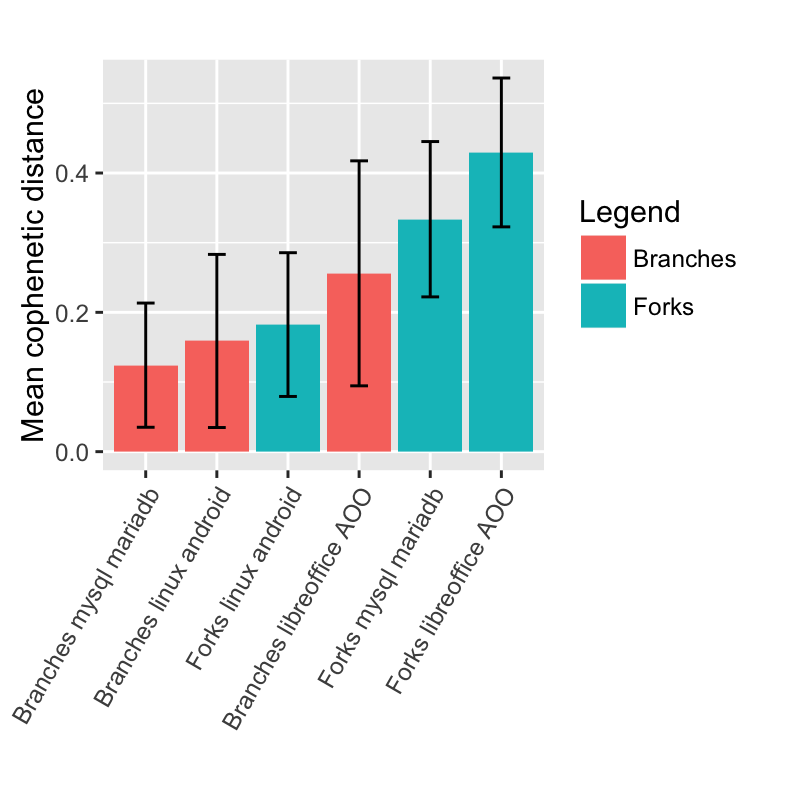
\includegraphics[width=\textwidth]{RQ1.png}
  \caption{Plot of the mean cophenetic distances between releases and their standard deviation for each fork case separately, sorted by distance.}
  \label{fig:rq1}
\end{figure}


Therefore, based on the three cases analysed, no generally applicable threshold value could be determined. Nevertheless, within a given forked project, the mean dissimilarity between releases on different forks is always larger than the mean dissimilarity between releases on the same branch. It can therefore be assumed that potential forks could be detected using this method.

\definition{RQ2}{Can the likely outcome (cooperation, competition or discontinuation) of an ongoing fork be predicted?}

The results for RQ2 are negative: the null hypothesis that forks with different outcomes are indistinguishable based on code and organizational measurements cannot be rejected. Consequently, no evidence could be found that the outcome of a project (i.e. “cooperation”, “competition” or “discontinued branch”) correlates with the distance between forks. Therefore, measurements of code and team characteristics are not sufficient to predict the outcome of a fork.

\subsection{Objective 5: Report}
The fifth objective was to report on the research for an audience of practitioners. Recommendations for practitioners are included in paragraph 4.4.

%----------------------------------------------------------------------------------------

\section{Interpretation in relation to the research aim}
The aim of the research was to assess whether methods and techniques from phylogenetics can be of real-world usefulness for the management of forks of open source software projects. 

\subsection{Forks as risks}
Research question 1 (RQ1) dealt with forks as a risk. If forks are a risk, then detecting development strands that are about to fork, before the actual fork happens, can be helpful to prevent the fork. The result for RQ1 provide evidence that, based on the three examples of forked projects examined, it is possible to detect a potential fork by examining the cophenetic distance matrix of the releases within a project. However, no generally applicable threshold could be determined beyond which any project would be likely to fork. Therefore phylogenetic methods are useful to detect potential forks, although to a lesser extent than expected.

\subsection{Forks as opportunities}
Research question 2 (RQ2) dealt with forks as opportunities. If the outcome of a fork can be predicted, then a purposeful fork could be used to solve technical, political or license problems. The result for RQ2 did not provide evidence that the outcome of a fork can be predicted solely based on measurements of code churn, team composition, edit frequency and code ownership. Therefore phylogenetic methods based on these measurements are not sufficient to predict the outcome of a fork.

\subsection{Tree thinking}
Phylogenetic trees are a depiction of estimated evolutionary relationships and could potentially be used to depict the state of a forked software project. This is illustrated in figure \ref{fig:example_tree1}, showing an example phylogenetic tree, constructed by subsampling the data collected for the MySQL / MariaDB fork. 

\citet{Baum2008b} coined the term “tree-thinking” to sum up the skills required to interpret phylogenetic trees. Basic concepts of “tree-thinking” could be ported to computer science and help to communicate about software evolution in general and forking processes in particular. \citet{Baum2008b} list terms useful for conceptualizing the evolutionary relationships captured in phylogenetic trees:

\begin{description}
\dt{Relatedness}{According to \citet{Baum2008b}, the term “relatedness” is used in biology to describe the recency of common ancestry. Ported to software evolution, relatedness could refer to the number of software releases between a pair of releases and their last common ancestor. For example, in figure \ref{fig:example_tree1}, MariaDB 10.0.1 and MySQL 5.6.5 (highlighted in blue) are more related to each other through their common ancestor MySQL 5.0.0 (highlighted in green), than to the majority of releases within their respective projects.}

\dt{Clade}{In biological evolution, a clade is a group comprised of an ancestor and all its descendants \citep{Baum2008b}. In the study of software evolution, a clade could be defined as the release which introduced a feature and all subsequent releases. For example, in the MySQL/MariaDB fork depicted in figure \ref{fig:example_tree1}, the MySQL 5.6.11, MySQL 5.7 and MySQL 8 series branched at the same node (highlighted in purple), which suggests that they share one or more important features.}

\dt{Parsimony}{The principle of parsimony states that the most likely tree is the one which displays the data in the simplest way, i.e. the tree that implies the least number of evolutionary changes \citep{Baum2008b}. While this might not be what actually happened, the parsimony principle allows reducing complex relationships to a manageable size. Therefore, parsimony could be applied to depict and grasp the release history of complex software projects.  For example, in figure \ref{fig:example_tree1}, MySQL 8.0.0 (highlighted in yellow) is depicted as closely related to the MySQL 5.7 series.}

\dt{Convergent evolution}{Similarities between biological organisms can arise in unrelated clades as a result of convergent evolution \citep{Baum2008b}. In computer science, convergent evolution could be used to describe the situation that arises when unrelated software develops similar features. For example, several mobile operating systems have opted to distribute their software through an online "application store"; however, this does not imply that their source code stems from a common origin: as discussed in paragraph 4.1, the Android operating system is related to the Linux operating system; there are however other mobile operating systems (e.g. iOS) which are unrelated to Linux, but have opted for a similar "application store" distribution model.}
\end{description}

\begin{figure}[H]
  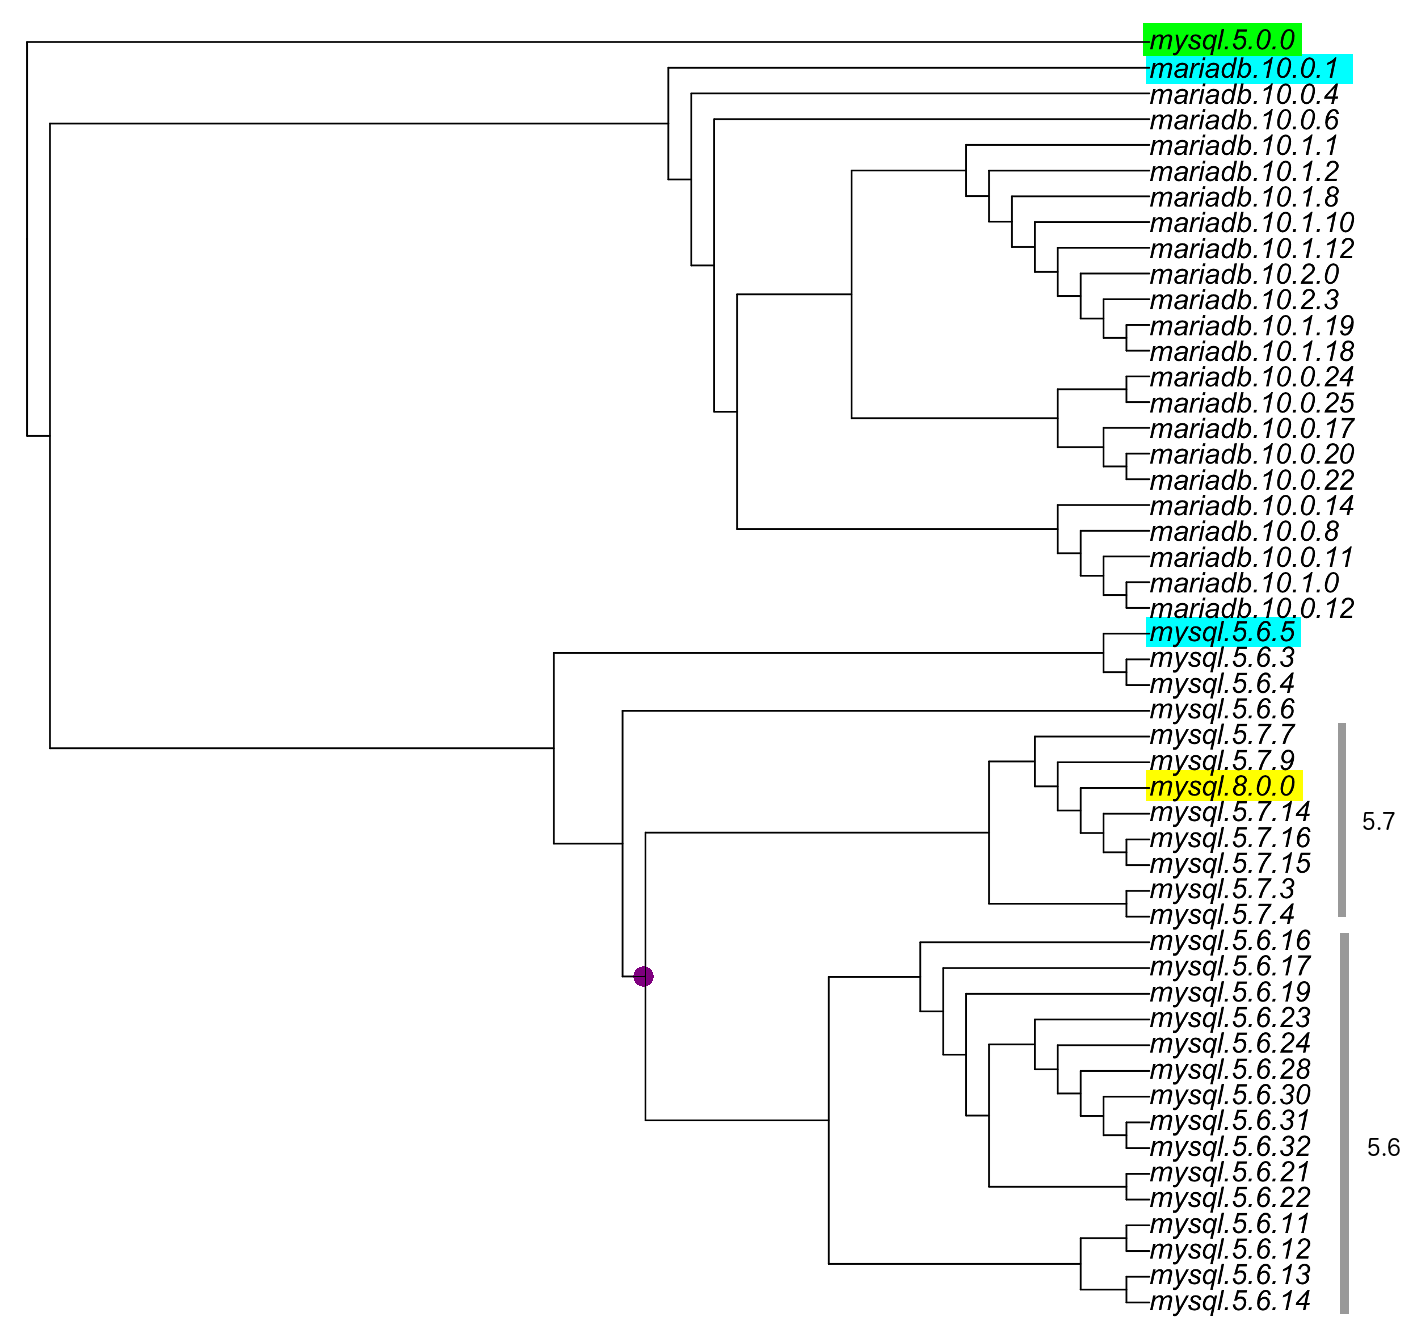
\includegraphics[width=\textwidth]{example_tree1.png}
  \caption{An example tree of the MySQL / MariaDB fork, obtained by subsampling fifty branches and ten thousand measurements.}
  \label{fig:example_tree1}
\end{figure}

%----------------------------------------------------------------------------------------

\section{Summary of Chapter 4}
Three forked open source projects were selected for carrying out case studies of forks with different reasons and outcomes. The three forks selected were: (1) MySQL server / MariaDB server, a database engine that forked due to licensing and community issues, (2) Linux kernel / Android kernel, a “friendly” fork, due to diverging commercial and technical strategies, and (3) Apache OpenOffice / LibreOffice, a fork due to the abandonment of the original project. 

Data was acquired from the online repositories of each project. Data was exported in a format suitable for analysis, re-encoded and cleaned-up where necessary. The previously discussed methods for estimating phylogenetic trees were implemented using the R language for statistical computing. It was determined that an analysis of the variance of the mean distances between branches and forks was a suitable statistical technique for answering the first research question (RQ1). The assumptions upon which this technique is predicated were checked. It was found that the Neighbour-Joining technique applied to the square root of the data was most likely to avoid false positives. Thereafter, it was determined that an analysis of the variance of the mean distances between forks with different outcomes, based on two data sets obtained from code-base and organizational measurements was a suitable statistical method for answering the second research question (RQ2). It was found that similar techniques as for RQ1 had to be applied to avoid false positives for RQ2. 

Interpretation yielded that branches can be told from forks within a project using methods for estimating phylogenetic trees, but no generally applicable threshold value between branches and forks could be determined. Therefore, the likelihood that a project will fork cannot be assessed with certainty. Nevertheless, branches that have wandered far away from the main development effort can be detected. No correlation could be found between the topology of the tree and the outcome of a fork, therefore the likely outcome of a fork cannot be foretold using these methods and measurements. An attempt was made at porting several concepts borrowed from biological evolution to describe relationships in software evolution.
 
%% Chapter 5

\chapter{Conclusions} % Main chapter title

\label{Chapter5} % For referencing the chapter elsewhere, use \ref{Chapter1} 

%----------------------------------------------------------------------------------------

\section{Conclusions about the objectives}
\subsection{Validity of the term “evolution” in the context of computer science}
The term “software evolution” has been used in computer science literature since the 1980s. However, as noted by several authors, the correspondence between biological and software evolution cannot be taken for granted. According to certain authors, “software evolution” is a metaphor at best, in any case, a discussion of software evolution should be grounded on a solid set of definitions: what entities are being studied, which measurement characters are suitable and which phylogenetic methods are applicable.

\subsection{Importance of forks}
The case studies selected substantiate that forking affects well-known projects with a large user base, and teams of more than thousand developers. Major software companies have used forking as a business strategy, leading to successful and failed projects. Therefore it is likely that forking has an impact on the software ecosystem, and its importance should not be underestimated.

\subsection{Applicability of phylogenetic trees to the study of software development}
As methods for estimating phylogenetic trees are quantifiable and repeatable, these methods provide a way to gain an objective understanding of the state of a fork. However, the research failed to provide a way to estimate the likely outcome of a fork. Nevertheless, the techniques used, matrices and trees, could be used by practitioners to gain an overview of the state of complex open source software development projects.

\section{Conclusions about the research aim}
\subsection{Choice of methods}
Methods from evolutionary biology were applied to answer the research questions. These methods purport to be repeatable and objective, two desirable qualities for any scientific method. In order to transfer these methods from biology to computer science while keeping these qualities intact, the correspondence between biological and software entities had to be made explicit: evolution is a process that affects a population of self-reproducing entities, and happens independently from the decisions taken by individual managers. The choice of methods was restricted by the fact that no unequivocal equivalent to biological genes could be found in the software domain: methods from evolutionary biology which are applicable to quantified characters of various kinds (“distance matrix” methods) were favoured, while methods limited to the examination of gene sequences had to be discarded.

\subsection{Vocabulary}
The chosen methods delivered a statistically significant result for the first research question, thus supporting the idea that, within the constraints defined above, these methods can be applied to software forks in particular and software development in general. A corollary of this is that terms used to describe biological evolution can be used to describe software evolution, thus the vocabulary of software development can be enriched. An attempt was made at redefining the following terms in the context of software development: clade, relatedness, convergent evolution and parsimony.

\subsection{Importance of additional factors}
Failing to obtain a positive result for the second research question shows that intrinsic characteristics of the code base and of the developer team are not sufficient to predict the outcome of a fork, therefore the outcome of a fork might be influenced to a great extent by other factors: the managerial, economic and social context of the project comes to mind.

\section{Further work}
Further work could be accomplished in several thematic areas:

\begin{description}
\dt{Socio-technical context}
\dd{As noted in the conclusions, this research suggests that additional factors, managerial, economic, social or otherwise, have an influence on the outcome of a fork. Finding a connection between the outcomes of forks and such factors could provide evidence as to the importance of these factors in a wider context within computer science.}

\dt{Validation and calibration}
\dd{This research found that forks can be distinguished from branches within the three projects analysed. It should be possible to repeat this analysis using additional examples to validate this result.}

\dt{Empirical studies of forks}
\dd{Any case-study of forked projects could potentially benefit from applying phylogenetic methods to visualize and quantify the forking process.}
\end{description}

\section{Implications of the research}
Best practices in software development recommend using a repository for keeping track of releases and versions of software. For example, the popular Github online service (http://github.org) provides free online repositories for open source projects, and the Gitlab project (http://gitlab.com) provides open source software intended for setting up a development environment for open source or commercial software development. 

However, tools for visualizing the state of branches, releases and forks are limited in scope. Practical implications of this research could be: (1) representing the history of a project using phylogenetic trees, which provide an easy to grasp overview of the state of development of a project. (2) Constructing a shaded distance matrix, which encodes pairwise dissimilarity of releases within a project using a colour scale: the lighter the shade, the greater the dissimilarity (an example shaded matrix is given in table 3.4). Based on the results for obtained for research question 1, a shaded distance matrix would be a suitable technique for detecting potential fork candidates. 

Such an implementation would have to overcome a number of technical difficulties, among which the prohibitively long computation time required for estimating a phylogenetic tree of a real-life project using the methods explored in this research is probably the most difficult to surmount. Computation time could be reduced by implementing the software in a compiled computer language, using a non-relational database to store the data and optimizing the algorithms used for calculating the distance matrix and for estimating the tree.

\section{Reflection on the experience of the research process}

\subsection{The choice of problem}
The primary aim of scientific research is to discover new knowledge, and the choice of a scientific problem is essential in achieving this aim: a good problem can be described in terms of feasibility and interest \citep{Alon2009a}. The chosen problem in this research was tackled by attempting to answer two research questions. The methods used to answer these questions are well-documented in literature and were implemented using existing software libraries, therefore the problem was relatively easy to solve. As the problem has a limited scope (forks of open source software), the increase in knowledge expected from answering these questions was also rather small. Therefore the chosen problem is of the easy and moderately interesting kind. A better problem would not be necessarily more difficult, but more interesting: for example expanding the scope of the research to applying phylogenetic techniques to the study of the governance of open source projects, instead of merely of forks, could potentially have yielded more interesting results.

\subsection{Transdisciplinarity}
A different way to increase the interest of the problem would be to look at the research as a study case in transdisciplinarity, i.e. porting methods from one scientific field (biology) into another (computer science). Some of the literature reviewed for this research is relatively old, e.g. \citet{Sneath1962a}, yet seems to be still relevant to computer science. This suggests that methods from one scientific field can have a second life in another field; therefore the lifecycle of scientific methods could be expanded. Such a research would however be beyond the limits of the qualification sought here.
 

%----------------------------------------------------------------------------------------
%	THESIS CONTENT - APPENDICES
%----------------------------------------------------------------------------------------

\appendix % Cue to tell LaTeX that the following "chapters" are Appendices

% Include the appendices of the thesis as separate files from the Appendices folder
% Uncomment the lines as you write the Appendices

% Appendix A

\chapter{Appendix A: Database schema} % Main appendix title

\label{AppendixA} % For referencing this appendix elsewhere, use \ref{AppendixA}

The database schema used to store the raw data collected from the software repositories studied is
documented in figure \ref{fig:appA_db_schema}.

\begin{figure}[H]
  \centering
  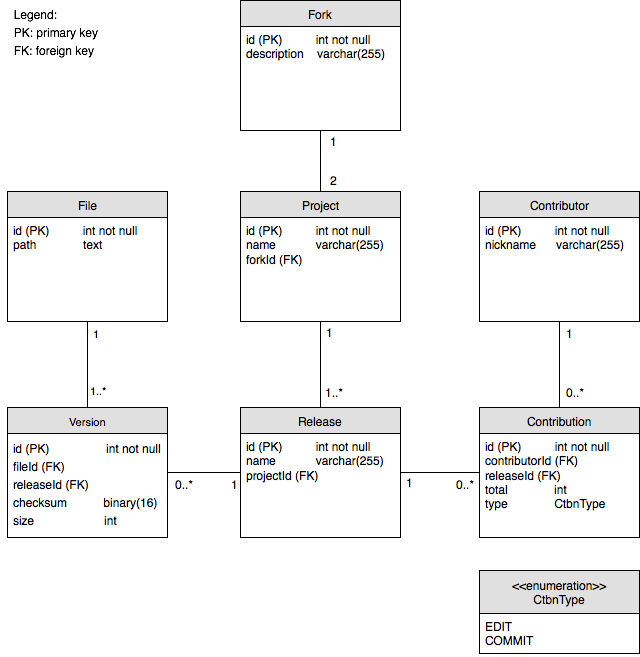
\includegraphics[width=\textwidth]{appA_db_schema.png}
  \caption{Database schema to hold data on forked repositories.}
  \label{fig:appA_db_schema}
\end{figure}


The database is composed of the following entities:
\begin{itemize}
  \item{One \textbf{fork} per \textbf{forked project} (e.g. MySQL, MariaDB).}
  \item{Each \textbf{project} has several \textbf{releases} (e.g. MySQL 5.5, MariaDB 10.0 ...).}
  \item{Each release is composed of \textbf{versions} of \textbf{files}, e.g. the file /src/main.c may be present or absent in a given release.}
  \item{Code churn characteristics (3.1.1) are recorded for each file \textbf{version}.}
  \item{Team characteristics (3.1.1) are recorded for each \textbf{release} as the number of
\textbf{contributions} (edits and commits) per \textbf{contributor}.}
\end{itemize}
%% Appendix B

\chapter{Appendix B: Implemented Software} % Main appendix title

\label{AppendixB} % For referencing this appendix elsewhere, use \ref{AppendixA}

The software implemented for the research is documented in the class diagram in figure \ref{fig:appB_software}.

\begin{figure}[H]
  \centering
  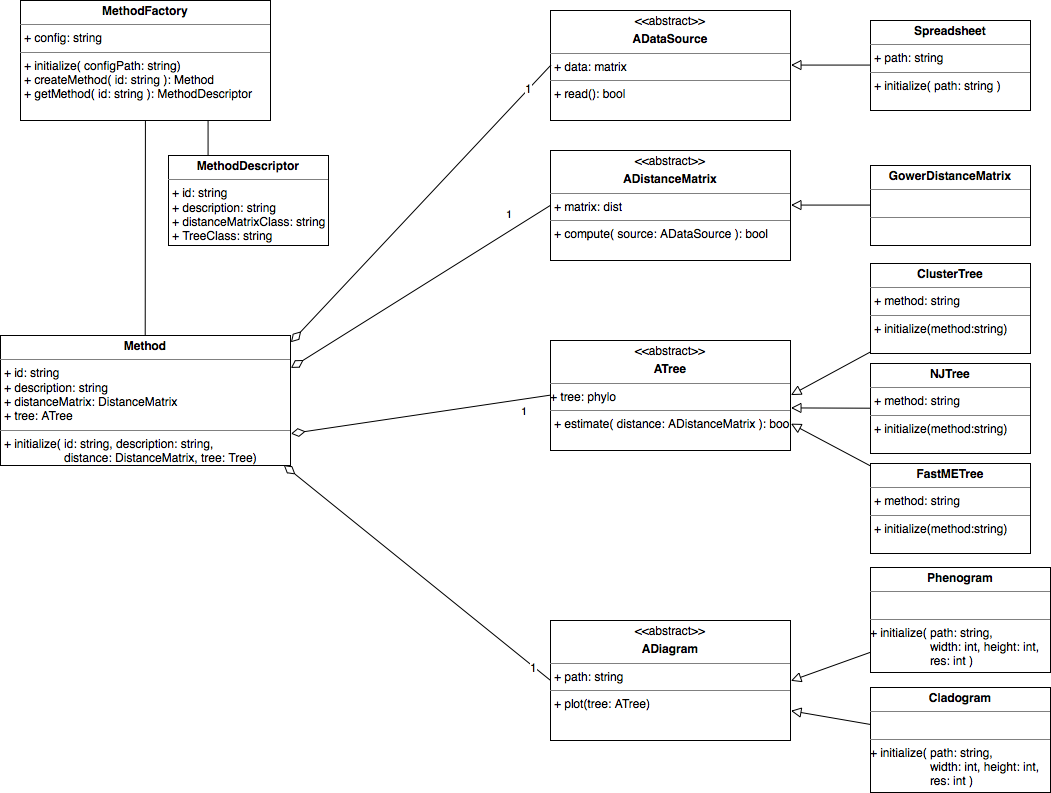
\includegraphics[width=\textwidth]{appB_software.png}
  \caption{Class diagram of the analysis software implemented for this research.}
  \label{fig:appB_software}
\end{figure}

\begin{itemize}
  \item{The \textbf{MethodFactory} takes a \textbf{MethodDescriptor} and creates a \textbf{Method} object. Method
descriptions are read from an XML configuration file. The method object aggregates a data
source, a distance matrix, a tree and a diagram objects.}
  \item{Objects extending \textbf{ADataSource} can read data exported from the database. \textbf{Spreadsheet} reads tabular data in "comma separated values" format.}
  \item{Objects extending \textbf{ADistanceMatrix} compute distances between branches.
\textbf{GowerDistanceMatrix} implements the techniques discussed in 3.1.2}
  \item{Objects extending \textbf{ATree} estimate phylogenies based on distance matrices. \textbf{ClusterTree}, \textbf{NJTree} and \textbf{FastMETree} implement the techniques discussed in 3.1.3.}
  \item{Objects extending \textbf{ADiagram} plot trees (“dendrograms”). \textbf{Phenogram} and \textbf{Cladogram} implement visualizations of taxonomic and cladistic relationships respectively.}
\end{itemize}
%\include{Appendices/AppendixC}

%----------------------------------------------------------------------------------------
%	BIBLIOGRAPHY
%----------------------------------------------------------------------------------------

\printbibliography[heading=bibintoc]

%----------------------------------------------------------------------------------------

\end{document}  
